\documentclass{article}

% Packages you should include
\usepackage[utf8]{inputenc}
\usepackage{amsmath, amssymb}   % Math support (optional)
\usepackage{graphicx}           % Optional, for figures
\usepackage{hyperref} 
\usepackage{subcaption} % For subfigure environment
\usepackage{stackengine}
\def\stacktype{L}

\usepackage{personal}
\usepackage[numbers]{natbib}
\bibliographystyle{plainnat}
\usepackage{wrapfig}
\usepackage{graphicx}
\usepackage{listings}
\usepackage{parskip}
%\lstset{numbers=left, frame=tblr, basicstyle=\tiny, tabsize=3}
\definecolor{codegreen}{rgb}{0,0.6,0}
\definecolor{codegray}{rgb}{0.5,0.5,0.5}
\definecolor{codepurple}{rgb}{0.58,0,0.82}
\definecolor{backcolour}{rgb}{0.95,0.95,0.92}

\lstdefinestyle{mystyle}{
    backgroundcolor=\color{backcolour},   
    commentstyle=\color{codegreen},
    keywordstyle=\color{magenta},
    numberstyle=\tiny\color{codegray},
    stringstyle=\color{codepurple},
    basicstyle=\ttfamily\footnotesize,
    breakatwhitespace=false,         
    breaklines=true,                 
    captionpos=b,                    
    keepspaces=true,                 
    numbers=left,                    
    numbersep=5pt,                  
    showspaces=false,                
    showstringspaces=false,
    showtabs=false,                  
    tabsize=2
}
\lstset{style=mystyle}


\begin{document}
\begin{titlepage}
\begin{center}
    \vspace{15cm}
    \huge{Semester Project}\\
    \vspace{2cm}
    \Huge{Compressive Sensing with Applications to Near-Field to Far-Field Antenna Pattern
Extrapolation}\\
    \vspace{2cm}
    \Large{Jonas Thalmeier}\\
    \vspace{1cm}
    30/04/2025
\end{center}
\vspace{3cm}
\begin{figure}[h]
    \centering
    
\includegraphics[width=.5\textwidth]{Figures/Eurecom.png}
\end{figure}
\end{titlepage}

\newpage
\tableofcontents
\thispagestyle{empty}
\newpage
\setcounter{page}{1}

\section{Introduction}
This semester project is carried out within the framework of the Data Science track of the Master program and is supervised by Prof. Dirk Slock, Dr. Zilu Zhao, and Dr. Fangqing Xiao. The project focuses on the theory and application of compressive sensing, a signal processing technique that allows for the recovery of sparse signals from undersampled measurements.

In the first phase (100-hour scope), the project explores state-of-the-art methods in compressive sensing, with particular attention to Sparse Bayesian Learning (SBL) and the use of Stein’s Unbiased Risk Estimate (SURE) for adaptive hyperparameter tuning in the SBL prior. Theoretical understanding and simulation-based validation on synthetic data are key objectives of this part.

In the extended 200-hour version, the project further investigates the practical application of compressive sensing techniques to antenna pattern extrapolation, specifically in transitioning from near-field to far-field measurements. This includes the construction of appropriate dictionaries or sensing matrices, initially based on simplified analytical models of antenna radiation patterns.

\section{Synthetic Data Generation}

To evaluate the performance of the implemented algorithms in a controlled environment, synthetic data was generated following a standard compressive sensing model. The measurement vector $ \mathbf{t} \in \mathbb{R}^N $ is constructed as

\begin{equation}
    \mathbf{t} = \Phi \mathbf{w} + \mathbf{e},
\end{equation}

where $ \Phi \in \mathbb{R}^{N \times D} $ is a sensing matrix, $ \mathbf{w} \in \mathbb{R}^{D} $ is a sparse signal, and $ \mathbf{e} \in \mathbb{R}^{N} $ is additive Gaussian noise with standard deviation $ \sigma $.

The sensing matrix $ \Phi $ is constructed by selecting $ N $ rows at random from a normalized $ D \times D $ discrete Fourier transform (DFT) matrix. Optionally, a random Gaussian matrix with variance $1/N$ can be used instead of the DFT for comparison purposes.

The sparse vector $ \mathbf{w} $ contains a user-defined fraction $ \rho \in (0, 1) $ of non-zero entries. These entries are assigned random values drawn from a standard normal distribution, and their indices are randomly selected. The noise vector $ \mathbf{e} $ is sampled from a Gaussian distribution $ \mathcal{N}(0, \sigma^2) $.

This setup allows flexible control over the number of measurements $ N $, signal dimensionality $ D $, sparsity level $ \rho $, and noise level $ \sigma $, providing a reproducible and interpretable environment for algorithmic evaluation. The generation process is deterministic under a fixed random seed, ensuring consistency across multiple runs.


\section{Choice of Algorithm}

In the early phase of this project, a central task was to select a suitable inference algorithm for sparse signal recovery. The field of \emph{Approximate Message Passing} (AMP) algorithms has seen considerable research activity in recent years, offering powerful and efficient solutions for compressive sensing problems. A concise yet comprehensive overview is provided in the tutorial by \citet{zou2022concise}, which summarizes key variants and their respective strengths.



However, AMP methods rely heavily on assumptions about the structure of the measurement matrix. As noted by \citet{zou2022concise}, AMP algorithms often fail to converge when the measurement matrix deviates from the independent and identically distributed (i.i.d.) sub-Gaussian regime. To address this limitation, modified approaches such as Orthogonal AMP (OAMP) have been proposed \citet{zou2022concise}, extending AMP's applicability to certain classes of unitarily-invariant matrices.

In the context of this project, the eventual goal is to apply compressive sensing to near-field to far-field antenna pattern extrapolation. The underlying sparse representation may involve FFT bases or modal decompositions of the near-field, which are expected to yield structured, non-random measurement matrices. To maintain flexibility in handling such structure, methods constrained to i.i.d. random matrices—such as classical AMP—appear less suitable.

As a result, I chose to explore an alternative inference approach based on the Expectation Maximization (EM) algorithm, as introduced by \citet{wipf2004sparse} first. The EM-based SBL framework is known for its robustness and generality, making fewer assumptions about the measurement matrix. While it may not offer the same computational efficiency as AMP in ideal settings, it provides a more versatile and stable foundation for the anticipated applications of this project.

\section{EM-Based Sparse Bayesian Learning}

To estimate sparse weights from an overcomplete basis, the Expectation-Maximization (EM) algorithm proposed in \citet{wipf2004sparse} was implemented. This method belongs to the broader Sparse Bayesian Learning (SBL) framework, where sparsity is induced not by fixed priors, but through evidence maximization over a parameterized Gaussian prior.

\subsection{Model Overview}

Given an observation model
\begin{equation}
    \mathbf{t} = \Phi \mathbf{w} + \boldsymbol{\epsilon}, \quad \boldsymbol{\epsilon} \sim \mathcal{N}(0, \sigma^2 \mathbf{I}),
\end{equation}
where $\mathbf{t} \in \mathbb{R}^N$ is the observed signal, $\Phi \in \mathbb{R}^{N \times D}$ is the (possibly overcomplete) measurement matrix, and $\mathbf{w} \in \mathbb{R}^D$ is the weight vector to be estimated, SBL assumes a zero-mean Gaussian prior with individual variances for each weight:
\begin{equation}
    p(\mathbf{w} ; \boldsymbol{\gamma}) =\prod\limits^M_{i=1}(2\pi\gamma_i)^{-\frac{1}{2}}\exp (-\frac{w_i^2}{2\gamma_i}).
\end{equation}
The hyperparameters $\boldsymbol{\gamma}$ (the prior variances of the weights) are inferred via Type-II maximum likelihood by marginalizing out $\mathbf{w}$ and maximizing the resulting evidence.

\subsection{Algorithm Description}

The EM algorithm alternates between computing the posterior distribution over weights (E-step) and updating the hyperparameters (M-step). Specifically:

\paragraph{E-step:}
The posterior $p(\mathbf{w} \mid \mathbf{t}, \boldsymbol{\gamma}, \beta)$ is Gaussian:
\begin{align}
    \boldsymbol{\Sigma}_w &= \left( \beta \Phi^\top \Phi + \mathrm{diag}(\boldsymbol{\gamma}^{-1}) \right)^{-1}, \\
    \boldsymbol{\mu}_w &= \beta \boldsymbol{\Sigma}_w \Phi^\top \mathbf{t},
\end{align}
where $\beta = 1/\sigma^2$ is the precision of the Gaussian likelihood.

\paragraph{M-step:}
The prior variances are updated based on the posterior moments:
\begin{equation}
    \gamma_i = \mu_{w,i}^2 + (\Sigma_w)_{ii},
\end{equation}
and the noise variance is updated as:
\begin{equation}
    \sigma^2 = \frac{1}{N} \| \mathbf{t} - \Phi \boldsymbol{\mu}_w \|^2 + \frac{1}{N} \sum_i (\Phi \Sigma_w \Phi^\top)_{ii}.
\end{equation}
In my implementation, the update of $\sigma^2$ was simplified or deferred for stability, and a fixed $\beta$ was used initially.

\subsection{Implementation Remarks}

The algorithm was implemented in Python based directly on the formulation in \citet{wipf2004sparse}. A simplified version of the EM loop is shown below:

\begin{verbatim}
mu, Sigma = estimate_posterior()
gamma = mu**2 + np.diag(Sigma)
\end{verbatim}

The evolution of weights was tracked during training for diagnostic purposes, and convergence is monitored using the maximum change in $\mu$ and the relative mean squared error with respect to $\mathbf{t}$.

The main practical limitation of this approach lies in the need to invert a $D \times D$ matrix at every iteration to compute $\Sigma_w$, making it computationally expensive for high-dimensional problems. This is noted in the original paper as well \cite[p.~2155]{wipf2004sparse}, and future work may include reformulating the algorithm to reduce this complexity using the Woodbury identity or low-rank approximations.

\subsection{Scalability via Covariance-Free Expectation Maximization (CoFEM)}

While the EM-based Sparse Bayesian Learning implementation performs well for small-scale problems, it becomes prohibitively slow as the problem size increases. This is due to the need to invert a dense $ D \times D $ matrix in each iteration to compute the posterior covariance. To address this computational bottleneck, the \emph{Covariance-Free EM (CoFEM)} algorithm as proposed by \citet{lin2022covariance} was implemented.

CoFEM avoids explicitly computing or storing the posterior covariance matrix. Instead, it estimates the required posterior statistics—the mean vector $ \boldsymbol{\mu}_w $ and the diagonal elements of the covariance matrix $ \Sigma_{jj} $—by solving a set of linear systems involving the precision matrix. These estimates are obtained using Rademacher probe vectors and linear solvers such as conjugate gradient, allowing for significant computational and memory savings.

In the E-step, the algorithm solves one linear system to compute the posterior mean and $ K $ additional systems to estimate the posterior variances using the diagonal estimation rule. The M-step then updates the hyperparameters $ \alpha_j $ using the standard SBL update:

\begin{equation}
    \alpha_j = \frac{1}{\mu_j^2 + s_j},
\end{equation}

where $ \mu_j $ is the $ j $-th component of the posterior mean and $ s_j $ is the estimated variance of $ w_j $ obtained from the Rademacher probe-based approximation.

Although the CoFEM algorithm is designed to benefit from conjugate gradient (CG) solvers for efficiently handling large-scale linear systems, the custom CG implementation used in this project proved to be slower than expected. In practice, it exhibited slower convergence and higher runtime compared to NumPy’s built-in direct solver.. As a result, the final implementation resorts to NumPy’s \texttt{np.linalg.solve} for solving the linear systems in the E-step, which yielded higher performance for the problem sizes considered in this study.

To assess the scalability, the runtime of the EM and CoFEM algorithm was measured as a function of the number of measurements $ N $, with parameters set as follows:  $ D = 3N $, sparsity level $ \rho = 0.1 $, and noise variance $ \sigma^2 = 10^{-6} $. The algorithms iterated until the relative residual dropped below 1e-2:
\begin{equation}
\frac{|\mathbf{t} - \Phi \boldsymbol{\mu}|_2}{|\mathbf{t}|_2} < 10^{-2}
\end{equation}
Both algorithms required roughly the same numbers of iterations.

As shown in Figure \ref{fig:runtime_comparison}, the CoFEM implementation significantly reduces runtime compared to the standard EM approach, especially as the dimensionality increases.

\begin{figure}[H]
    \centering
    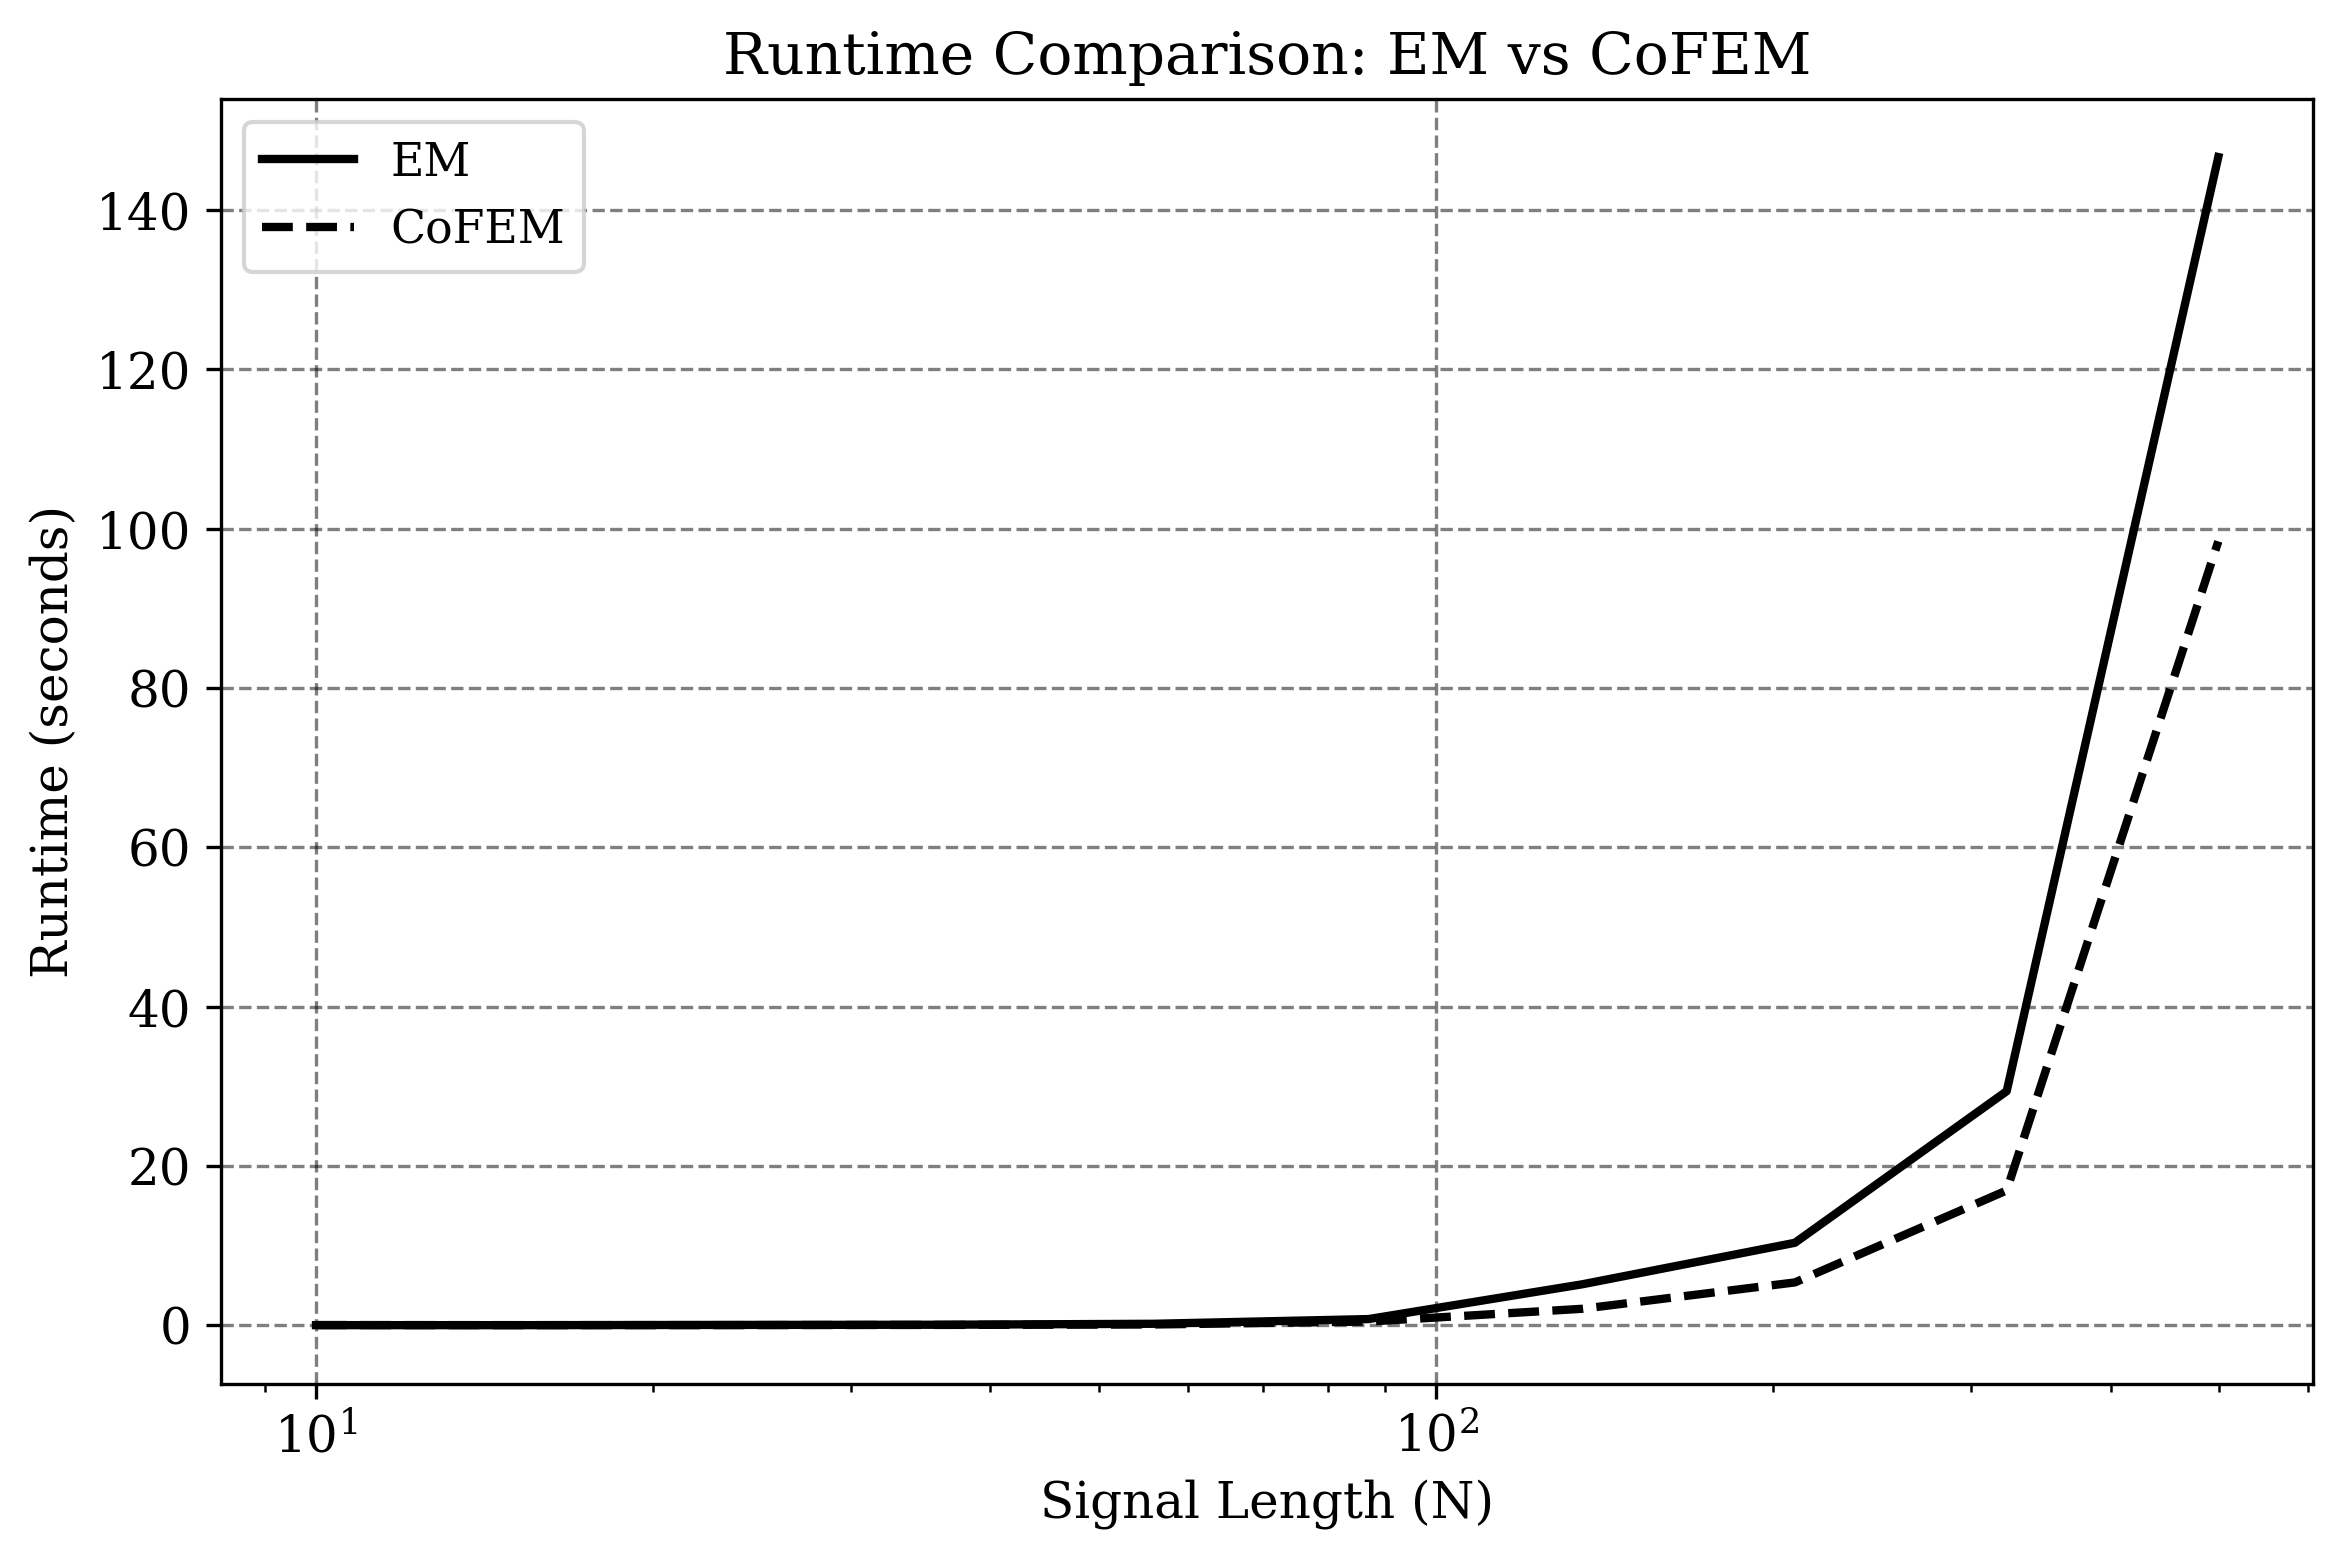
\includegraphics[width=0.75\textwidth]{Figures/runtime_comp.png}
    \caption{Runtime of the EM and CoFEM algorithms for increasing number of measurements $ N $. The dictionary size is set to $ D = 3N $.}
    \label{fig:runtime_comparison}
\end{figure}

While the CoFEM algorithm achieves a noticeable speedup over the standard EM algorithm—98.4 seconds compared to 146.6 seconds for N=500—the improvement falls short of the expected at least twofold acceleration.

\subsection{Performance Comparison of EM Algorithms}
\paragraph{Gaussian Matrix}
\label{sec:PerfEMCoFEMGauss}
To compare the performance of different EM-based Sparse Bayesian Learning algorithms, experiments were conducted using synthetic data generated from Gaussian dictionaries, varying both the sparsity level $ \rho $ and the undersampling factor $ \delta = N/D $. Four variants were considered: standard EM and CoFEM, each with known and unknown noise variance. The normalized root mean squared error (NRMSE) was used to evaluate reconstruction quality. Results are averaged over multiple random trials to ensure statistical robustness.

The signal dimension was fixed to $ D = 1024 $. For the sparsity analysis the undersampling factor was fixed at $ \delta = 0.25 $, corresponding to $ N = \lfloor \delta D \rfloor $ measurements. For the undersampling analysis, the sparsity level was fixed at $ \rho = 0.06 $. The measurement matrix was drawn from a standard Gaussian distribution. Additive Gaussian noise with standard deviation $ \sigma = 0.01 $ was added to the measurements. For each setting, the reported results represent the average over five random trials to account for variability due to random initialization and noise.

As shown in Figure \ref{fig:accuracy_vs_sparsity} and Figure \ref{fig:accuracy_vs_undersampling}, all four algorithms exhibit remarkably similar performance across the full range of tested sparsity and undersampling settings. In particular, the CoFEM algorithm with unknown noise variance performs on par with the variants that assume knowledge of the noise level. This observation is consistent with the findings reported in \citet{lin2022covariance}, where CoFEM and EM methods were shown to yield nearly identical reconstruction accuracy under equivalent settings.

\begin{figure}[H]
    \centering
    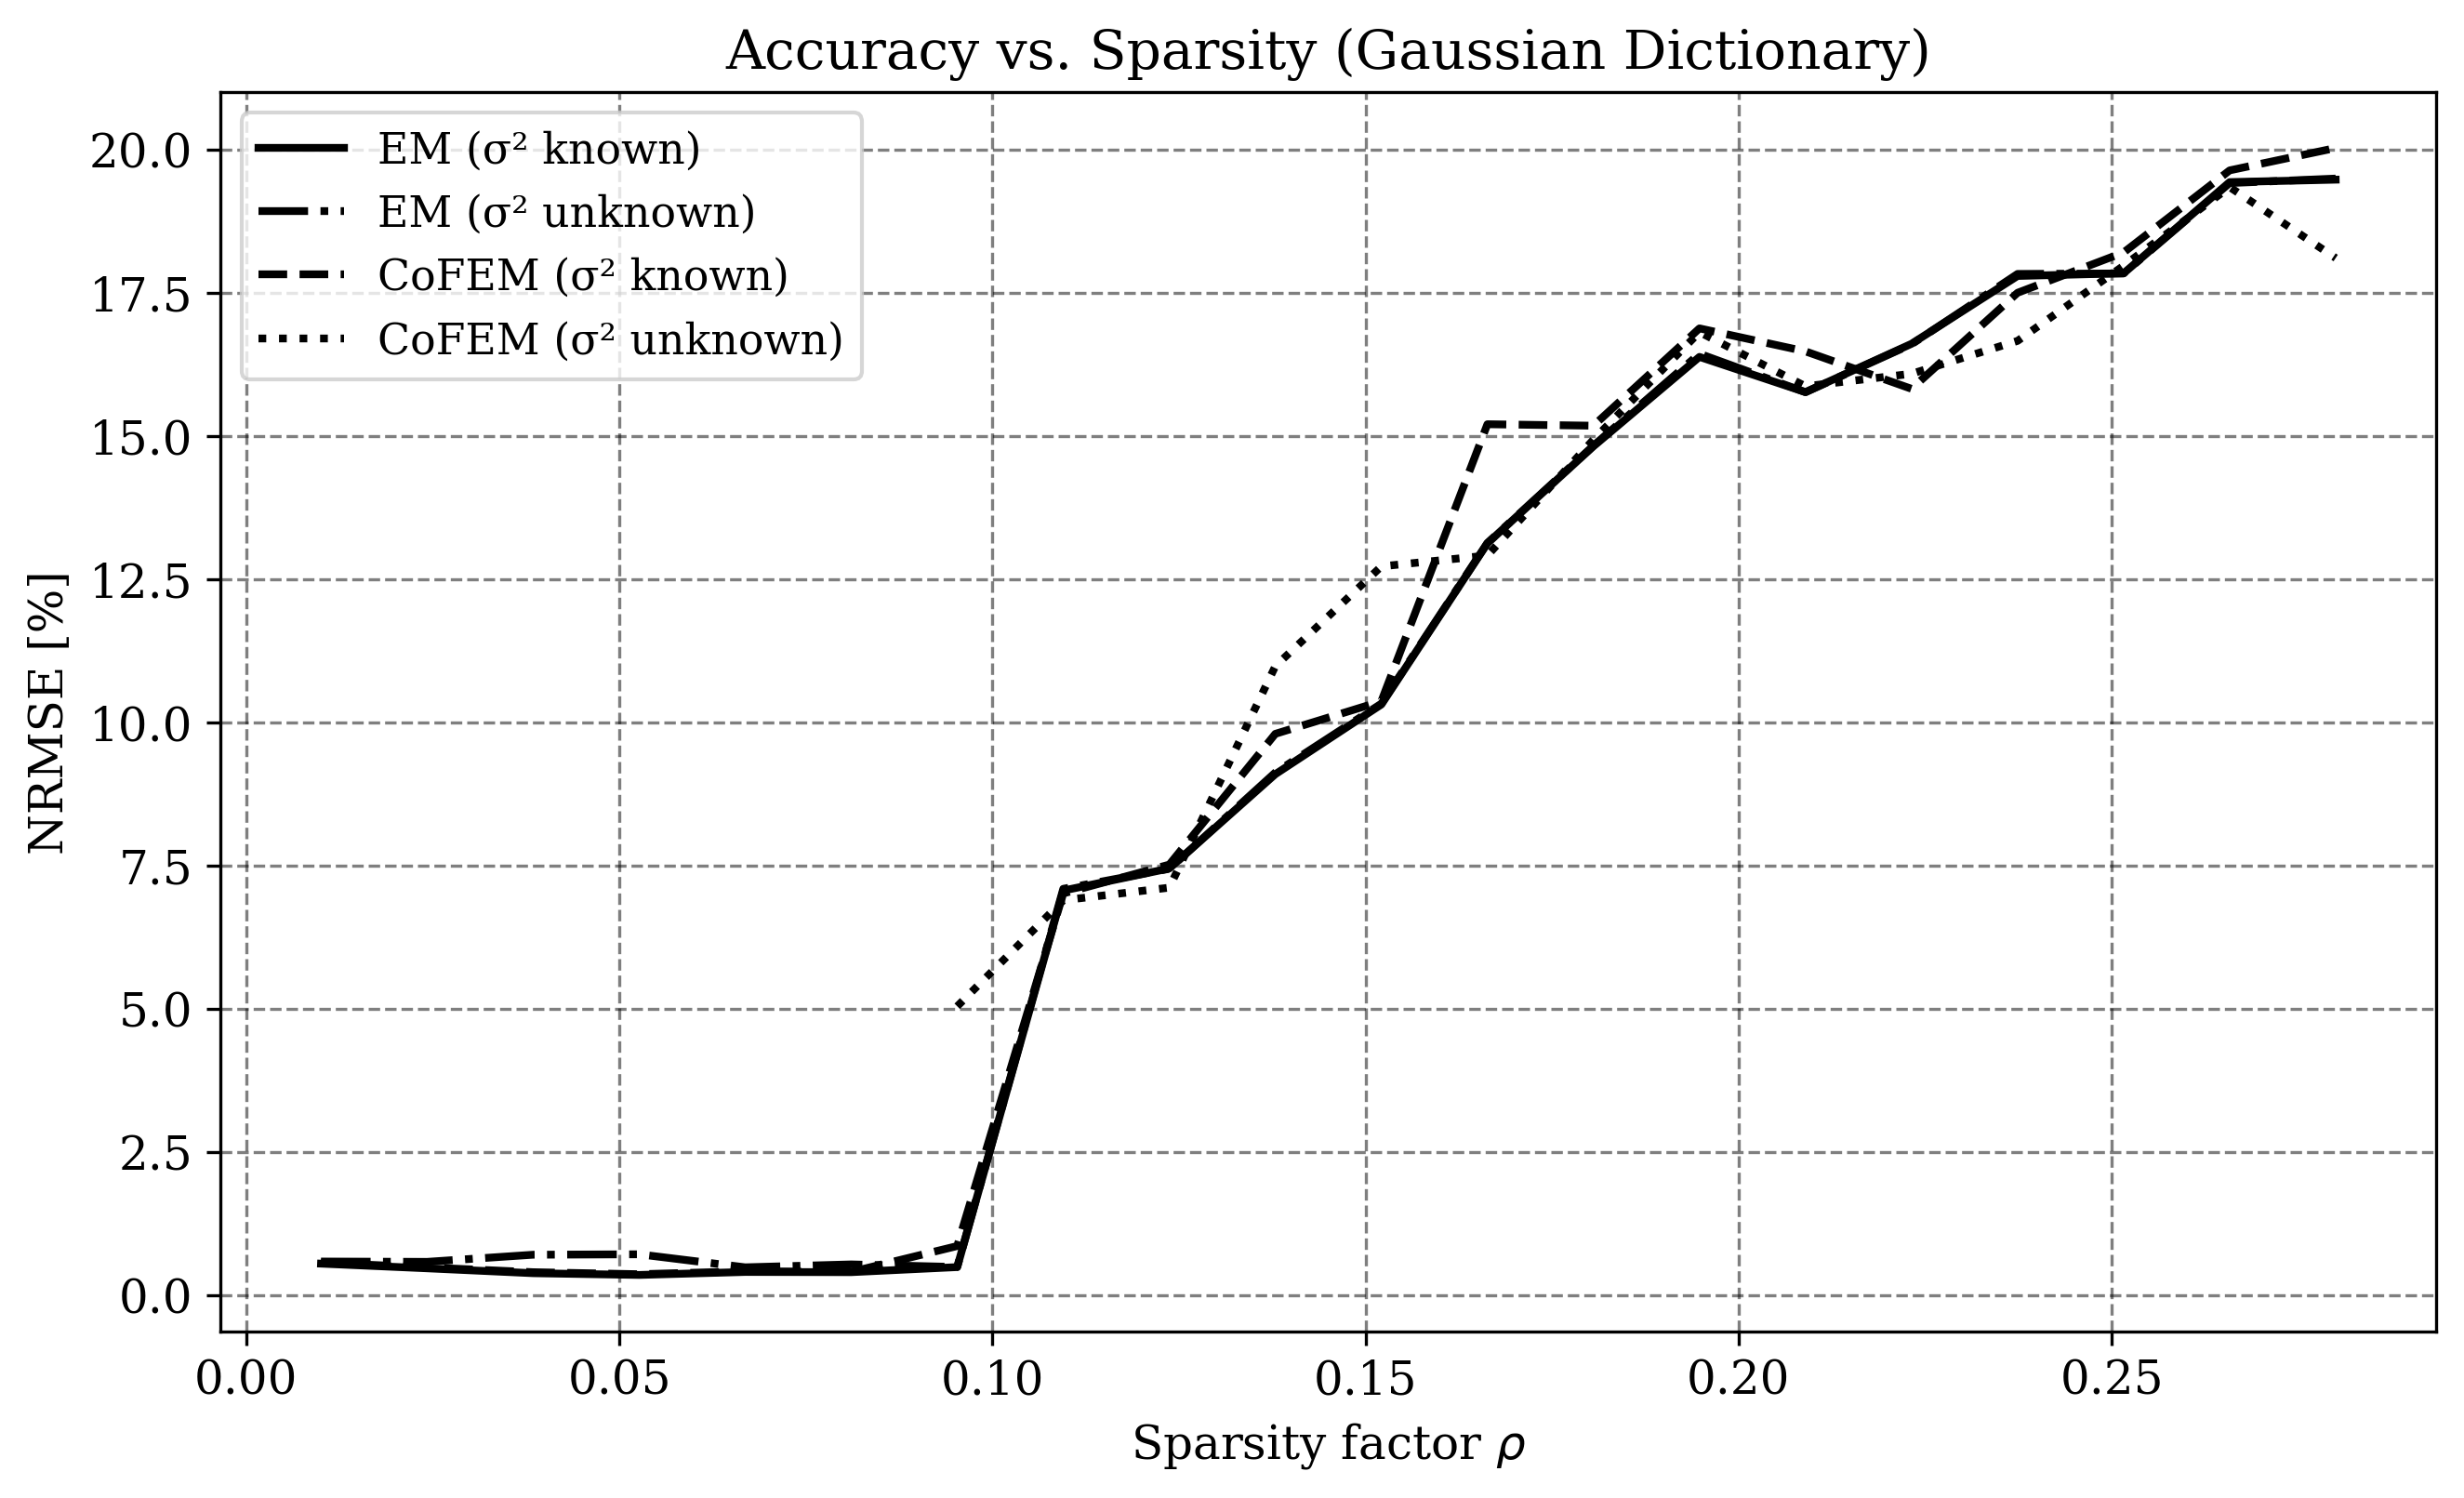
\includegraphics[width=0.75\linewidth]{Figures/accuracy_vs_sparsity_EMCoFEM.png}
    \caption{Reconstruction accuracy (NRMSE) versus sparsity level $ \rho $. All four EM variants show near-identical behavior.}
    \label{fig:accuracy_vs_sparsity}
\end{figure}

\begin{figure}[H]
    \centering
    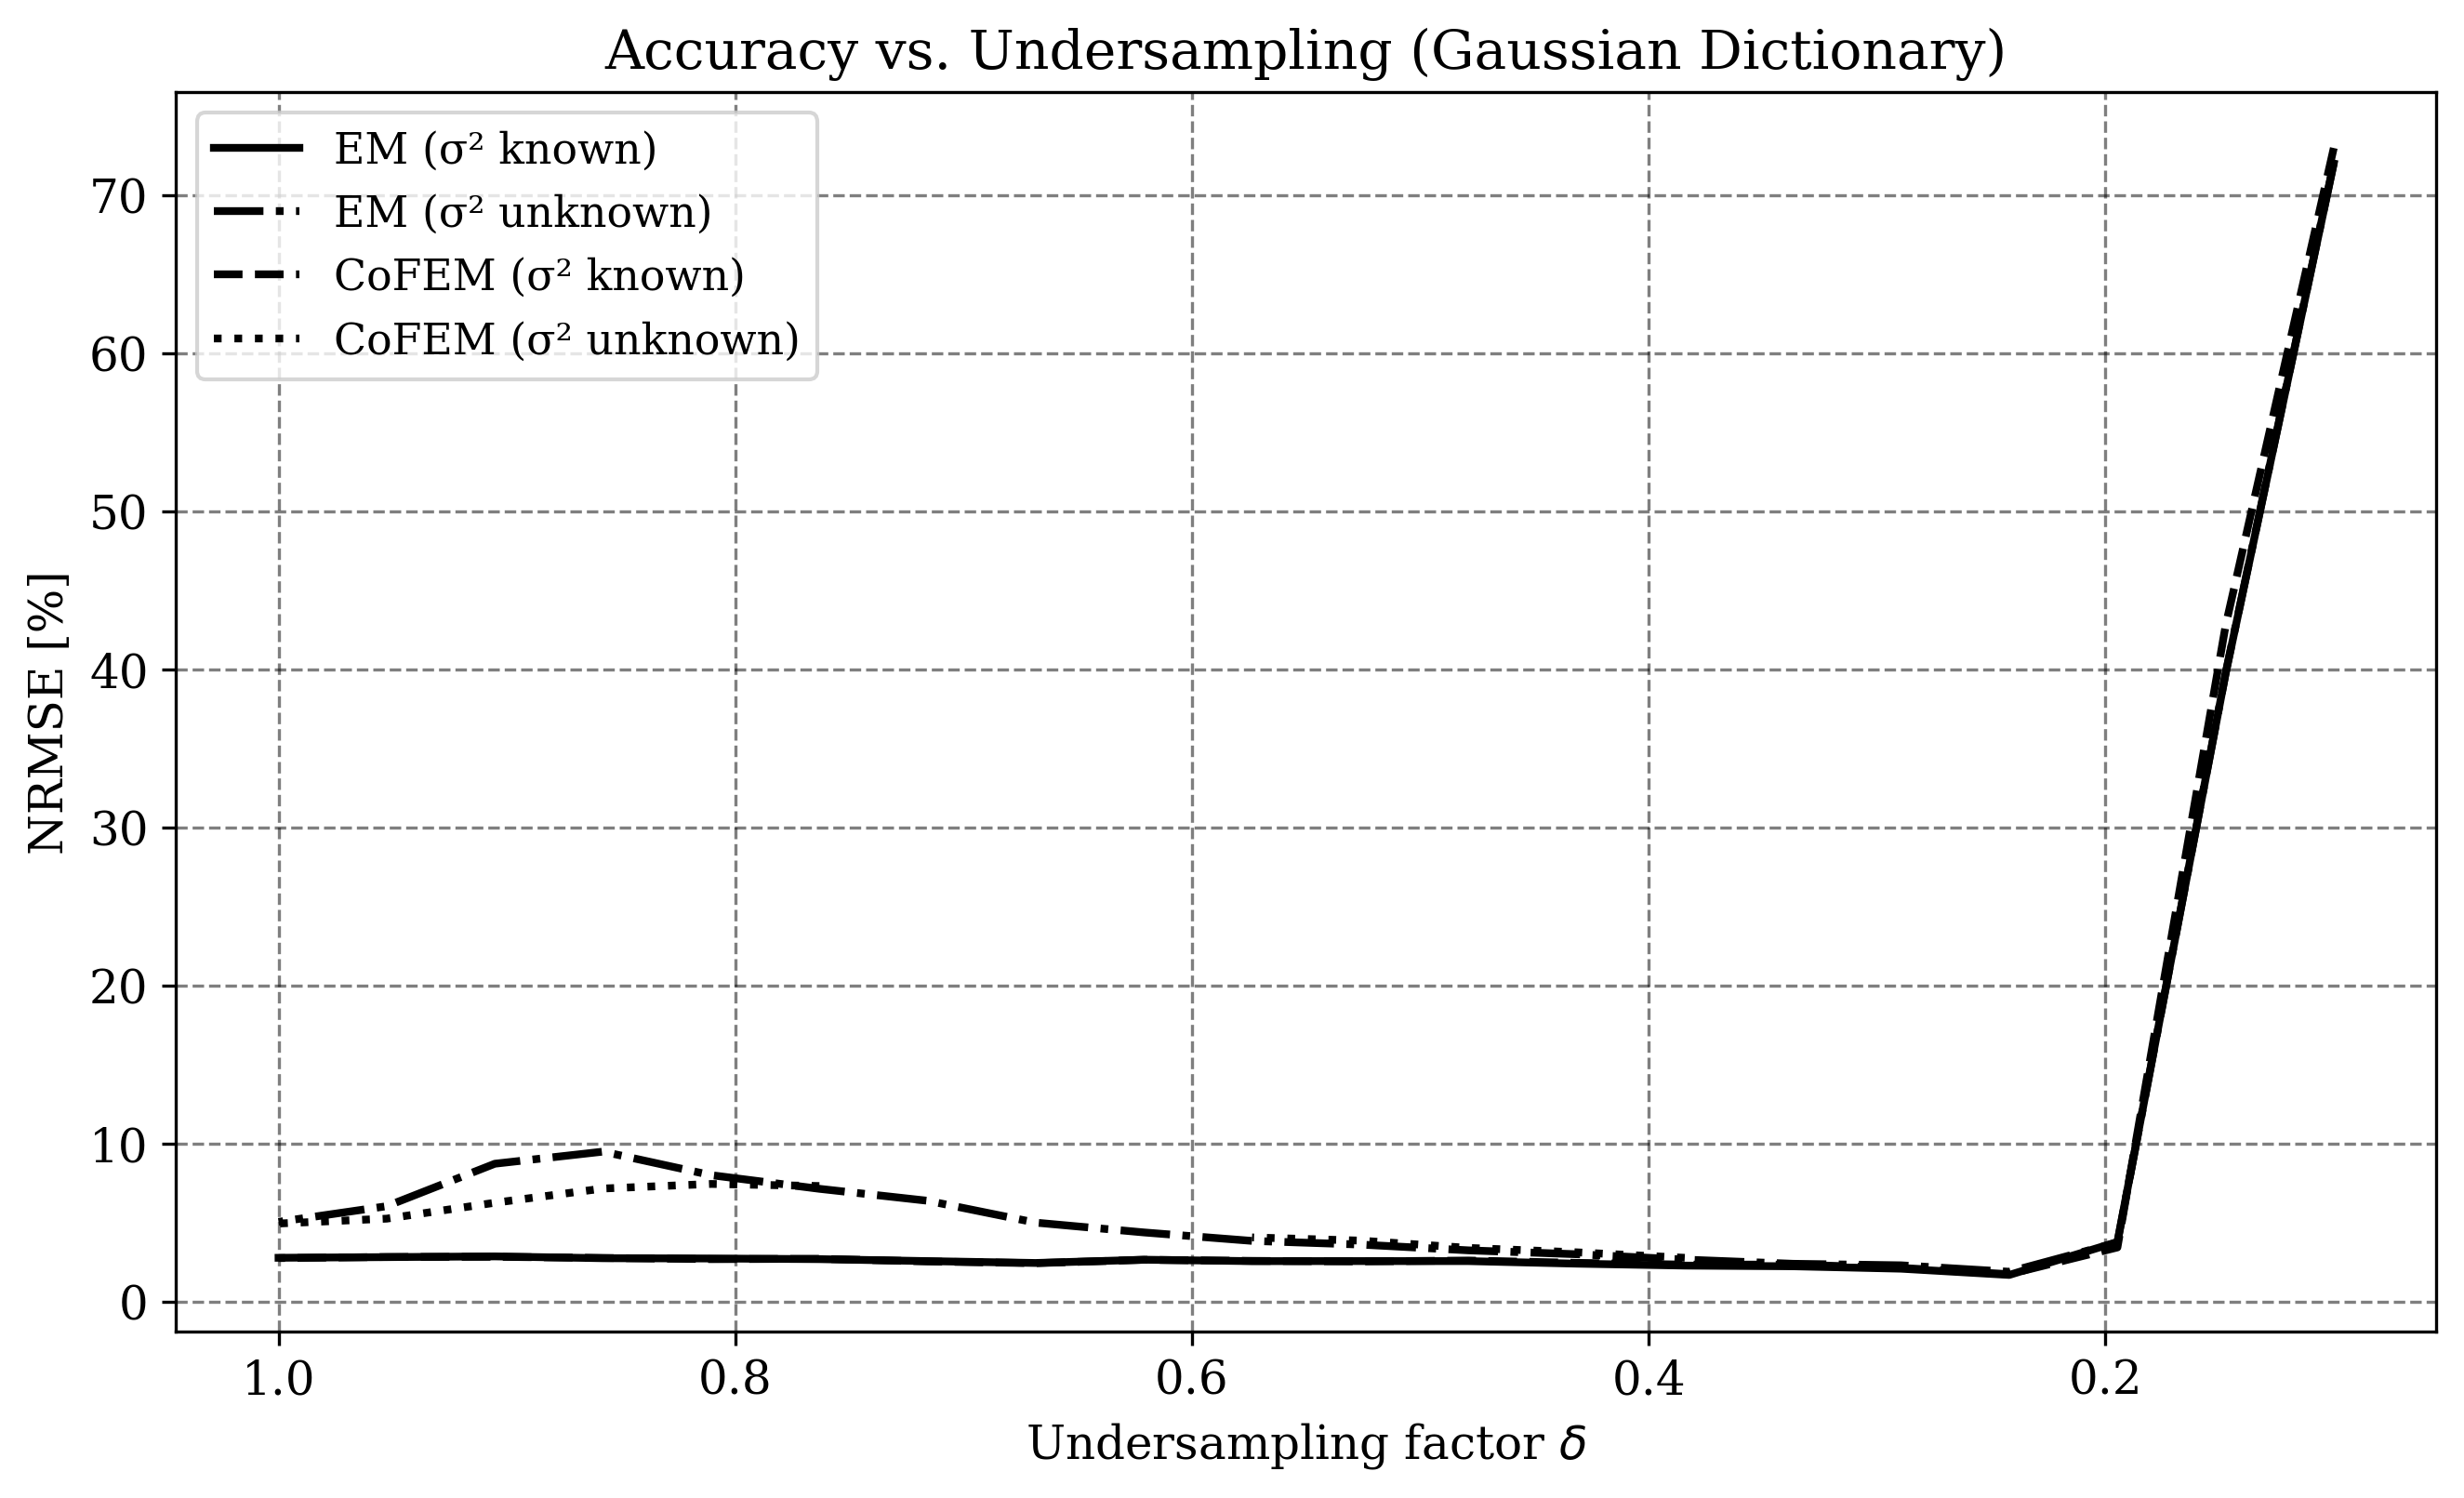
\includegraphics[width=0.75\linewidth]{Figures/accuracy_vs_undersampling_EMCoFEM.png}
    \caption{Reconstruction accuracy (NRMSE) versus undersampling factor $ \delta $. Similar performance is observed across all algorithms.}
    \label{fig:accuracy_vs_undersampling}
\end{figure}


Given these results, and in order to simplify subsequent analysis, I choose to focus on the CoFEM algorithm with unknown noise variance in the remainder of this report. This choice is motivated by its computational scalability, the practical advantage of not requiring prior knowledge of the noise level, and the observation that its reconstruction performance closely matches that of other EM-based approaches in the tested settings. While this similarity may not generalize to all scenarios, it provides a reasonable basis for concentrating on a single representative method in this context.


\paragraph{Fourier Matrix}
When the measurement matrix $\Phi$ is changed from a Gaussian random matrix to one representing a subsampled Fourier transform, several complications arise. Both the EM and CoFEM algorithms were adapted accordingly, replacing standard transposes with conjugate transposes and applying further minor modifications to support complex-valued inputs. Multiple approaches were explored to enable accurate diagonal estimation within the CoFEM framework under complex-valued settings; however, none of them yielded satisfactory results.

Despite these efforts, the EM algorithm continued to show unstable behavior. The initialization of the hyperparameter vector $\boldsymbol{\alpha}$ was found to significantly influence the outcome. In some instances, the algorithm converged to solutions with accuracy comparable to those obtained in the Gaussian matrix setting (Figure \ref{fig:accuracy_vs_sparsity_EM_gaussFFT}). In other cases, however, it resulted in drastically increased MSE values (Figure \ref{fig:accuracy_vs_undersampling_EM_gaussFFT}). This instability, combined with the sensitivity to initialization, rendered the EM approach unreliable for complex-valued measurement matrices.

In contrast, the algorithm described in Section \ref{sec:SBL_SURE}, which incorporates Sparse Bayesian Learning with SURE-based hyperparameter optimization, demonstrated more stable and consistent performance in the complex-valued setting. As a result, further efforts to adapt the EM algorithm for this case were discontinued.


\begin{figure}[H]
    \centering
    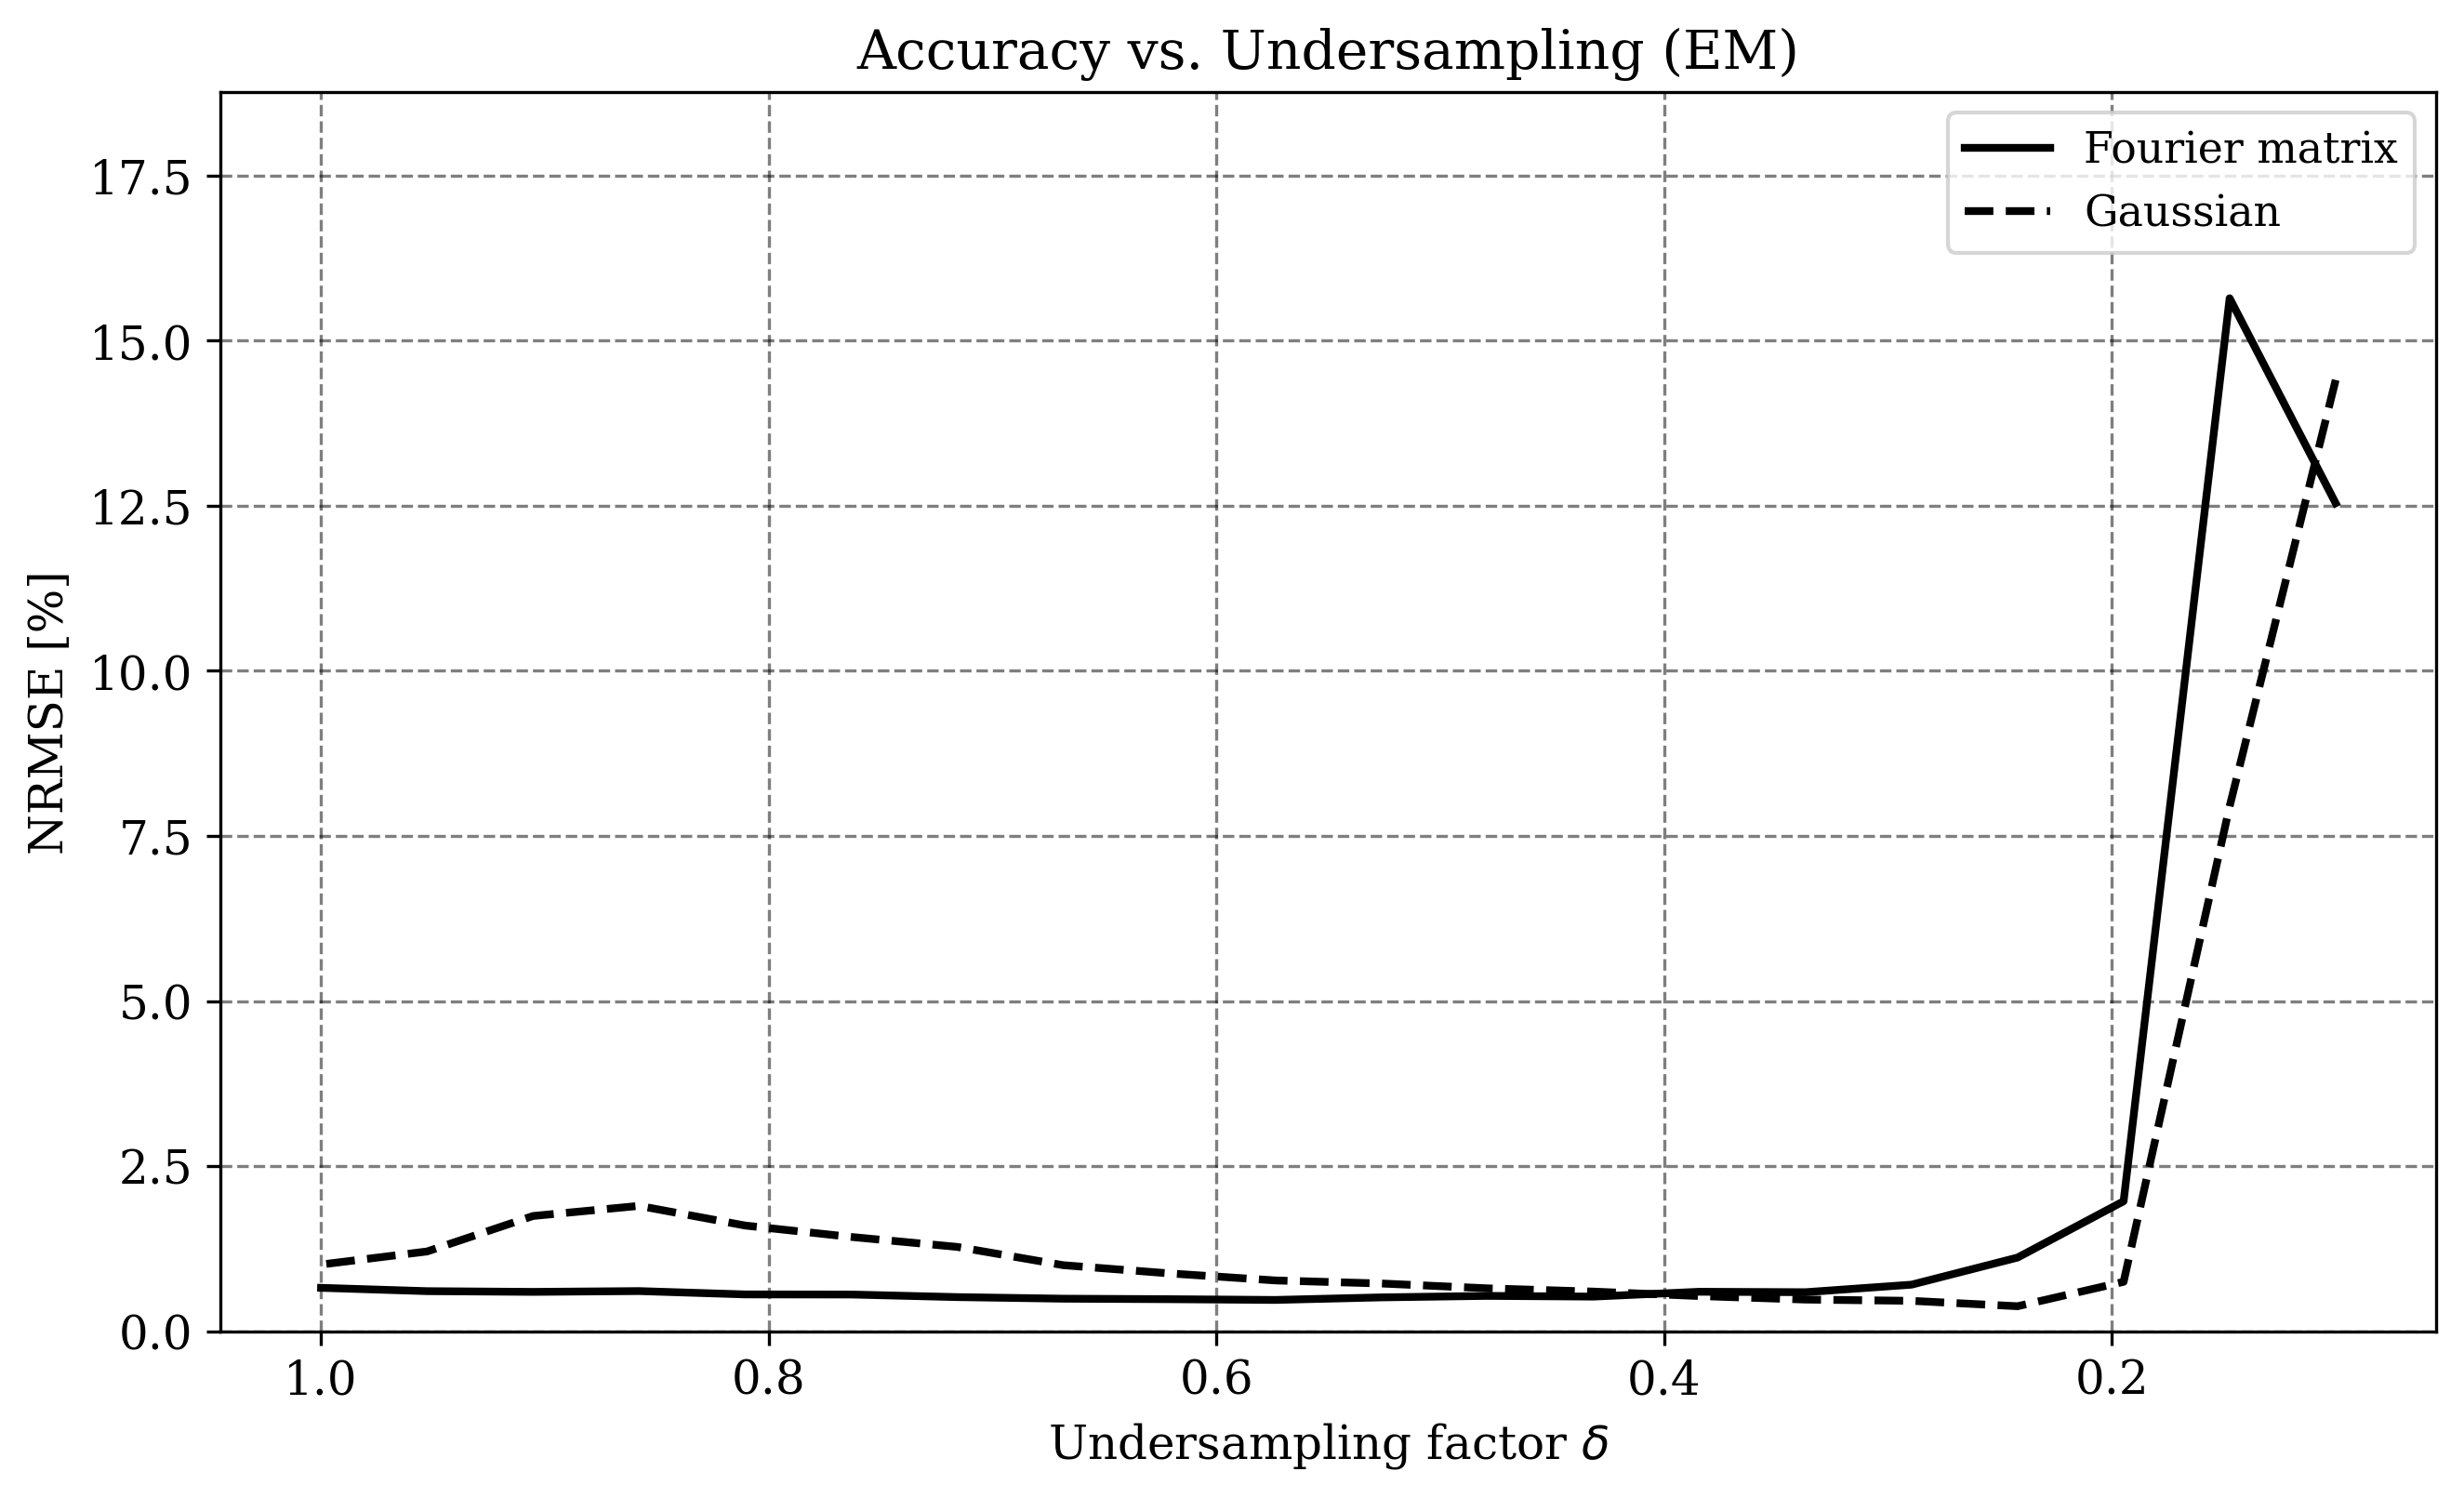
\includegraphics[width=0.75\linewidth]{Figures/accuracy_vs_undersampling_FFTGauss_EM.png}
    \caption{Reconstruction accuracy (NRMSE) versus undersampling factor $ \delta $.}
    \label{fig:accuracy_vs_undersampling_EM_gaussFFT}
\end{figure}

\begin{figure}[H]
    \centering
    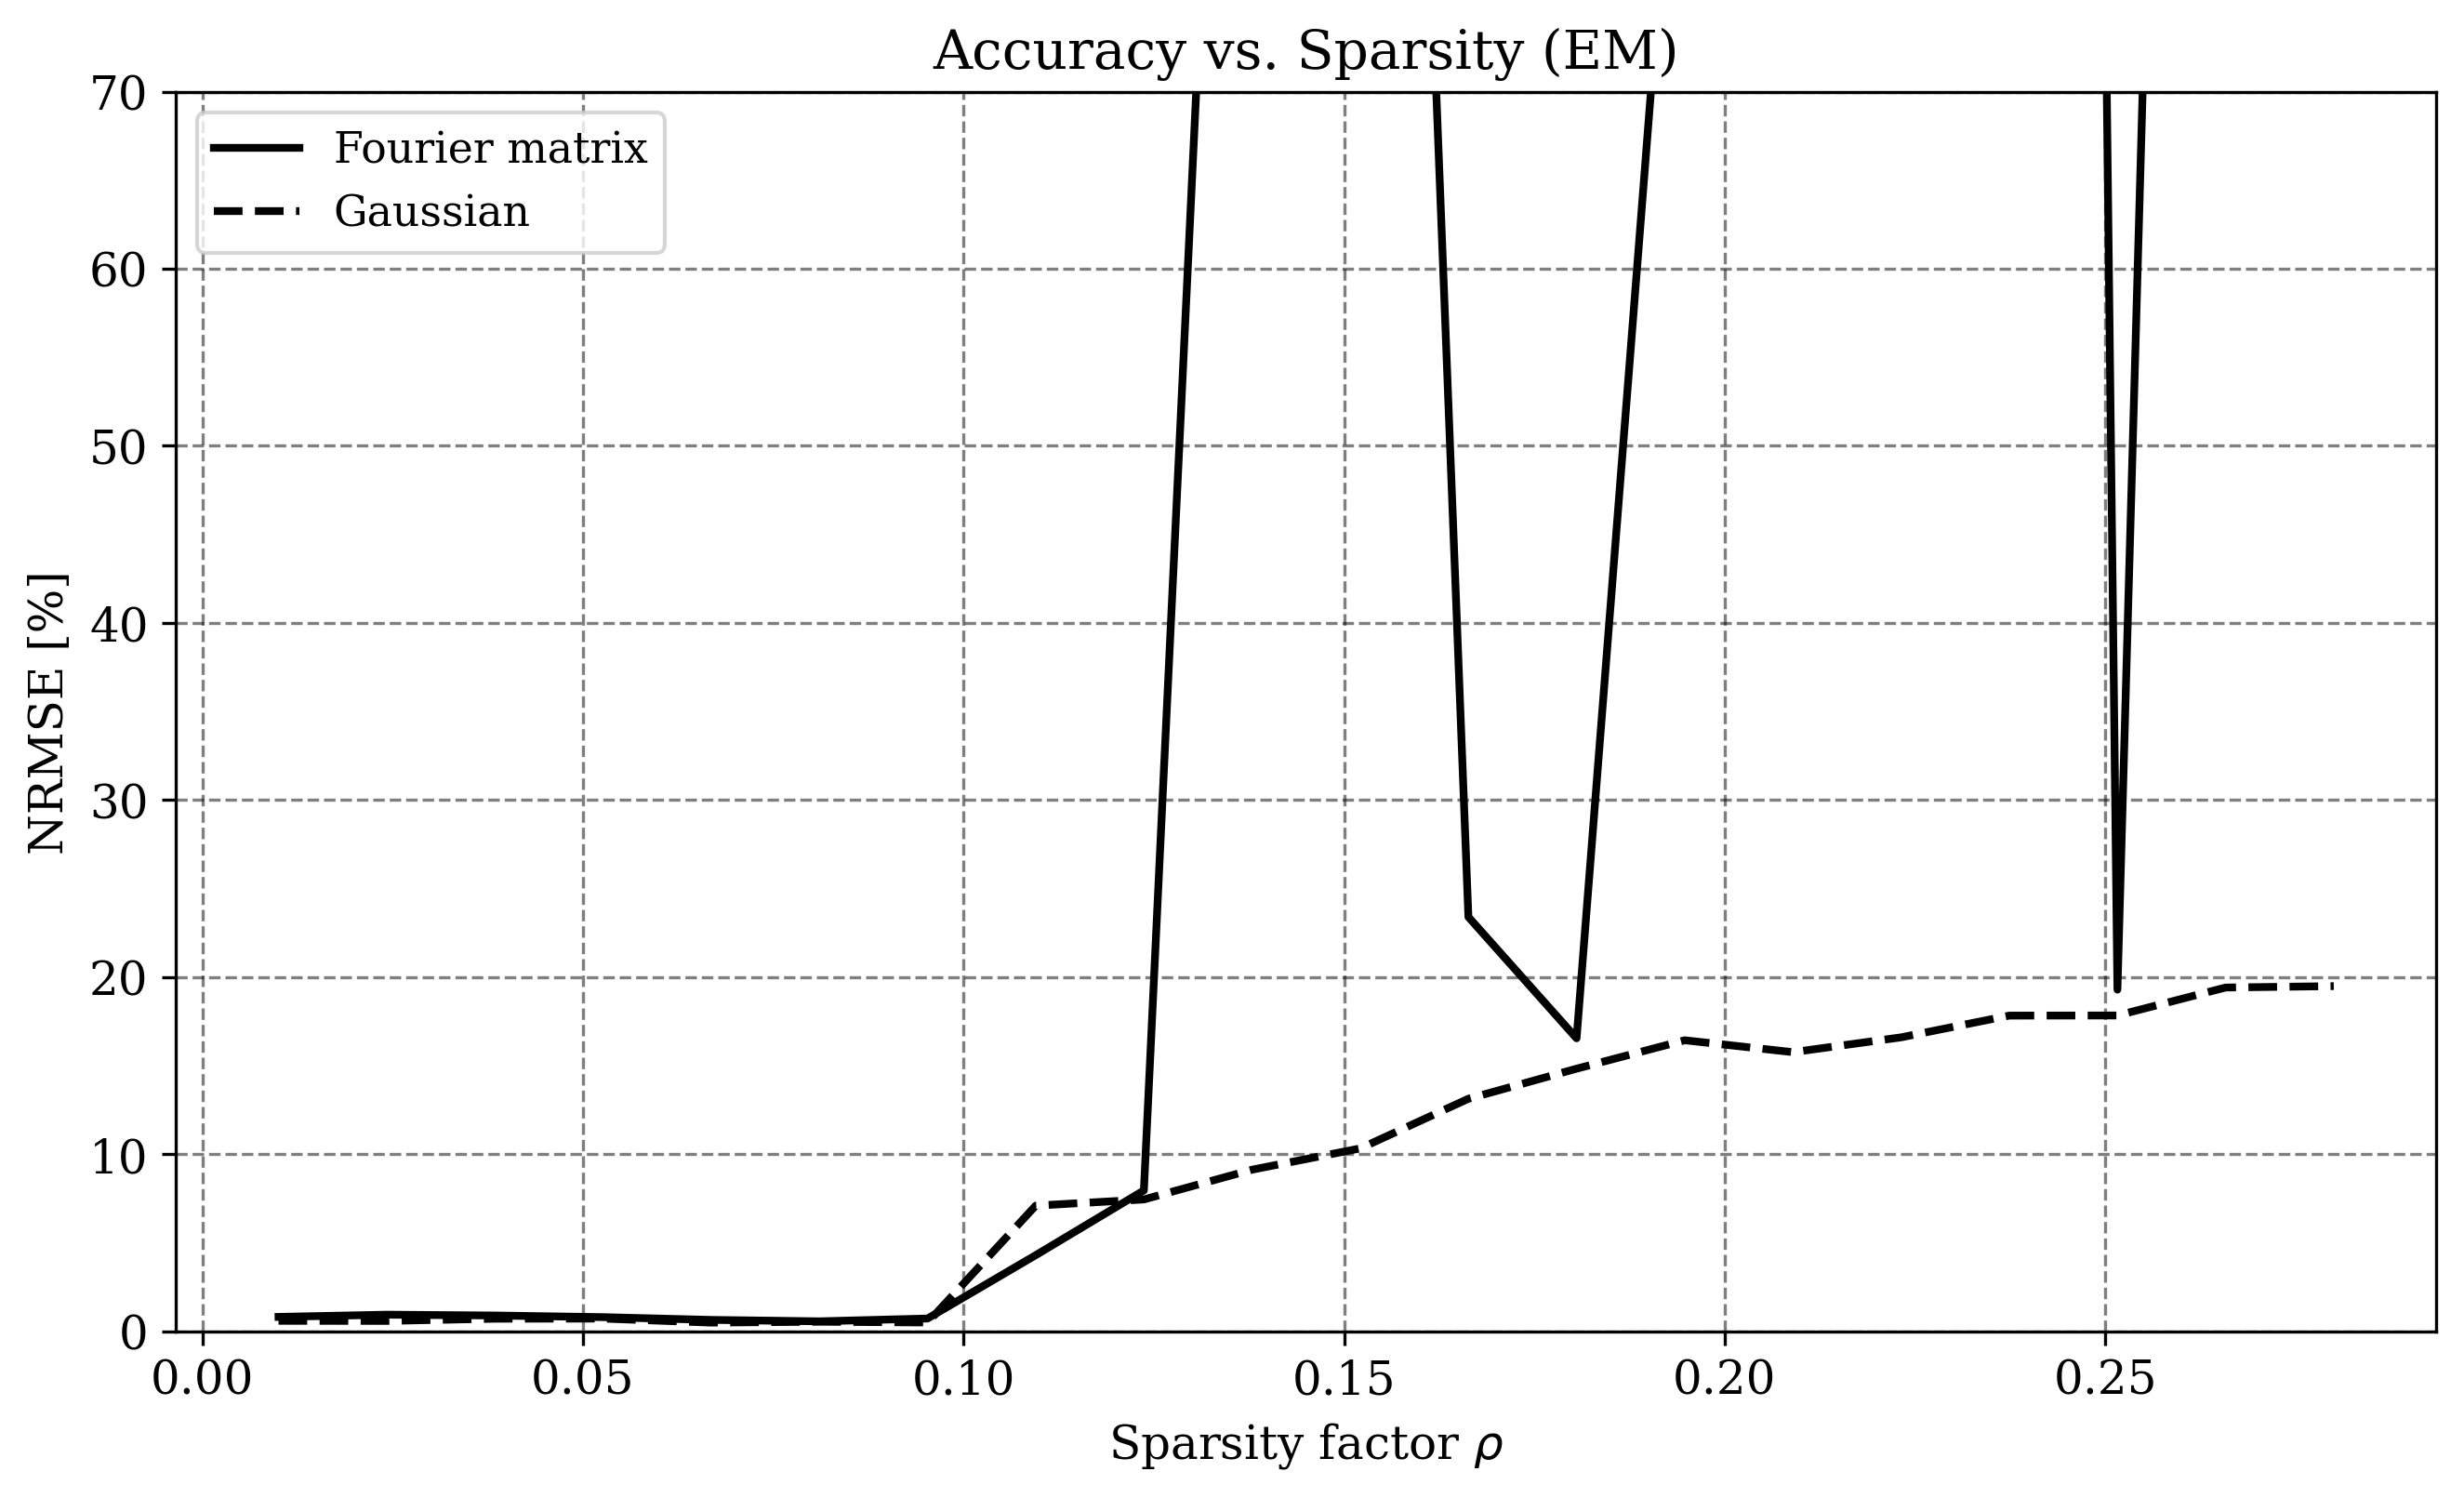
\includegraphics[width=0.75\linewidth]{Figures/accuracy_vs_sparsity_FFTGauss_EM.png}
    \caption{Reconstruction accuracy (NRMSE) versus undersampling factor $ \delta $.}
    \label{fig:accuracy_vs_sparsity_EM_gaussFFT}
\end{figure}


\section{Sparse Baysian Learning with Stein's Unbiased Risk Estimate}
\label{sec:SBL_SURE}
\subsection{Stein's Lemma}
Stein's Lemma provides a fundamental relationship between the expectation of a function of a Gaussian random variable and its derivative. For the univariate case, let $Z \sim \mathcal{N}(0, 1)$ and $f: \mathbb{R} \to \mathbb{R}$ be an absolutely continuous function with derivative $f'$ satisfying $\mathbb{E}|f'(Z)| < \infty$. Then, Stein's Lemma states:

\begin{equation}
    \mathbb{E}[Zf(Z)] = \mathbb{E}[f'(Z)]
\end{equation}

The proof follows from integration by parts and leverages the property of the standard normal density $\phi(z)$, where $\phi'(z) = -z\phi(z)$ (\citet{Tibshirani2015SteinS}). This result extends to $X \sim \mathcal{N}(\mu, \sigma^2)$ through standardization:

\begin{equation}
    \frac{1}{\sigma^2}\mathbb{E}[(X - \mu)f(X)] = \mathbb{E}[f'(X)]
\end{equation}

For the multivariate case, let $\mathbf{X} \sim \mathcal{N}(\boldsymbol{\mu}, \sigma^2 \mathbf{I}_n)$ and let $f: \mathbb{R}^n \to \mathbb{R}$ be an almost differentiable function with gradient $\nabla f$. Stein's Multivariate Lemma states:

\begin{equation}
    \frac{1}{\sigma^2}\mathbb{E}[(\mathbf{X} - \boldsymbol{\mu})f(\mathbf{X})] = \mathbb{E}[\nabla f(\mathbf{X})]
\end{equation}

This is proved by applying the univariate lemma component-wise and using Fubini's theorem under the almost differentiability condition \citet{Tibshirani2015SteinS}. The lemma enables covariance estimation without explicit knowledge of $\boldsymbol{\mu}$, replacing it with computable partial derivatives.

\subsection{Stein's Unbiased Risk Estimate (SURE)}
For a Gaussian model $\mathbf{y} \sim \mathcal{N}(\boldsymbol{\mu}, \sigma^2 \mathbf{I}_n)$ and estimator $\boldsymbol{\hat{\mu}}(\mathbf{y})$, the risk $R = \mathbb{E}\|\boldsymbol{\mu} - \boldsymbol{\hat{\mu}}\|_2^2$ can be decomposed as:

\begin{equation}
R = -n\sigma^2 + \mathbb{E}\|\mathbf{y} - \boldsymbol{\hat{\mu}}\|_2^2 + 2\sigma^2 \sum_{i=1}^n \text{Cov}(y_i, \hat{\mu}_i)
\end{equation}


Using Stein's Lemma, the covariance term is replaced with partial derivatives when $\boldsymbol{\hat{\mu}}$ is almost differentiable. This yields Stein's Unbiased Risk Estimate (SURE):

\begin{equation}
    \widehat{R} = -n\sigma^2 + \|\mathbf{y} - \boldsymbol{\hat{\mu}}\|_2^2 + 2\sigma^2 \sum_{i=1}^n \frac{\partial \hat{\mu}_i}{\partial y_i}(\mathbf{y})
\end{equation}

SURE provides an unbiased risk estimator ($\mathbb{E}[\widehat{R}] = R$) without requiring knowledge of $\boldsymbol{\mu}$ (\cite{Tibshirani2015SteinS}). For estimators depending on tuning parameters $\lambda$, SURE enables model selection through:

\begin{equation}
\hat{\lambda} = \underset{\lambda \in \Lambda}{\arg\min} \left( \|\mathbf{y} - \boldsymbol{\hat{\mu}}_\lambda\|_2^2 + 2\sigma^2 \sum_{i=1}^n \frac{\partial \hat{\mu}_{\lambda,i}}{\partial y_i}(\mathbf{y}) \right)
\end{equation}


This framework has become instrumental for risk estimation and hyperparameter optimization in high-dimensional statistics.

\subsection{Algorithm Design for SBL with SURE}
The implementation of Sparse Bayesian Learning (SBL) with Stein's Unbiased Risk Estimator (SURE) was planned based on the theoretical framework presented in \citet{slockSURE}. In this setting, we consider the linear model:

\begin{equation}
    \mathbf{y} = \mathbf{A}\mathbf{x} + \mathbf{v}, \quad \mathbf{v} \sim \mathcal{N}(\mathbf{v}; \mathbf{0}, \sigma^2 \mathbf{I}), \quad \mathbf{x} \sim \mathcal{N}(\mathbf{x}; \mathbf{0}, \mathbf{P}),
\end{equation}

where $\mathbf{y}$ represents the observed data, $\mathbf{A}$ is the measurement matrix, $\mathbf{x}$ is the sparse signal of interest, and $\mathbf{v}$ is additive Gaussian noise. The prior on $\mathbf{x}$ is Gaussian with covariance $\mathbf{P}$, which is typically diagonal to enforce sparsity. The posterior distribution of $\mathbf{x}$ given $\mathbf{y}$ is derived as:

\begin{equation}
    \mathbf{x}|\mathbf{y} \sim \mathcal{N}\left(\mathbf{x}; \mathbf{P}\mathbf{A}^T\mathbf{R}^{-1}\mathbf{y}, \mathbf{P} - \mathbf{P}\mathbf{A}^T\mathbf{R}^{-1}\mathbf{A}\mathbf{P}\right),
\end{equation}

where $\mathbf{R} = \mathbf{A}\mathbf{P}\mathbf{A}^T + \sigma^2 \mathbf{I}$. Alternatively, this can be rewritten as:

\begin{equation}
    \mathbf{x}|\mathbf{y} \sim \mathcal{N}\left(\mathbf{x}; \mathbf{S}^{-1}\mathbf{A}^T\mathbf{y}, \sigma^2 \mathbf{S}^{-1}\right),
\end{equation}

with $\mathbf{S} = \mathbf{A}^T\mathbf{A} + \sigma^2 \mathbf{P}^{-1}$. 

\subsection{Connection to Tipping's Fast Marginal Likelihood Algorithm}
The posterior expressions derived above align with the sparse Bayesian framework described in \citet{tipp2003fastsb}. By adopting the notation used in Tipping's paper, where $\mathbf{A} \rightarrow \boldsymbol{\Phi}$, $\mathbf{y} \rightarrow \mathbf{t}$, $\mathbf{x} \rightarrow \mathbf{w}$, and $\mathbf{P} \rightarrow \mathbf{A}^{-1}$, the posterior mean and covariance become:

\begin{equation}
    \boldsymbol{\mu} = \sigma^{-2}\boldsymbol{\Sigma}\boldsymbol{\Phi}^T\mathbf{t}, \quad \boldsymbol{\Sigma} = \left(\mathbf{A} + \sigma^{-2}\boldsymbol{\Phi}^T\boldsymbol{\Phi}\right)^{-1}.
\end{equation}

These expressions are identical to those derived in \citet{tipp2003fastsb} for the posterior distribution of the weights $\mathbf{w}$ in the sparse Bayesian learning framework. This equivalence confirms that the Fast Marginal Likelihood Maximisation algorithm proposed by Tipping can be directly applied to implement SBL with SURE in our setting.

The algorithm proceeds as follows:
\begin{enumerate}
    \item Initialize the hyperparameters $\boldsymbol{\alpha}$ and noise variance $\sigma^2$.
    \item Initialize the set of active basis $\mathcal{A}$ and compute the posterior statistics $\boldsymbol{\mu}$ and $\boldsymbol{\Sigma}$ using the current hyperparameters.
    \item Evaluate the marginal likelihood and update $\boldsymbol{\alpha}$ by sequentially adding, deleting, or re-estimating basis functions to maximize the marginal likelihood.
    \item Iterate until convergence, ensuring that the hyperparameters and noise variance are optimized for minimal mean squared error (MSE) as guided by SURE.
\end{enumerate}

This approach leverages the efficiency of Tipping's algorithm while incorporating the risk estimation principles of SURE to optimize hyperparameters. The result is a computationally tractable implementation of SBL that maintains sparsity and generalizes well, as demonstrated in the experiments reported in \citet{tipp2003fastsb}.

\subsection{Implementation of the Fast Marginal Likelihood Algorithm}

The Fast Marginal Likelihood Algorithm is implemented through an efficient basis selection and pruning strategy. Unlike traditional SBL approaches that update all basis functions simultaneously, this implementation sequentially evaluates individual basis functions to maximize the marginal likelihood more efficiently.

The algorithm begins by initializing a single most relevant basis function, selected by evaluating the correlation between each basis vector and the target signal. All other basis functions are initially deactivated by setting their corresponding $\alpha$ values to infinity. This sparse initialization provides a computationally efficient starting point.
    \begin{equation}
    \begin{split}
    \boldsymbol{\alpha_i} &= \infty \\
    \sigma^2 &= 1/\beta = 0.1\sigma^2_{\boldsymbol{t}} \\
    \theta_i &= \frac{\|\phi_i^* t\|}{\Re\{\phi_i^*\phi_i\}} \\
    \mathcal{A} &= \underset{i}{\arg\max} \theta_i \\
    \alpha_{i\in\mathcal{A}} &= \frac{\Re\{\phi_i^*\phi_i\}}{\theta_i-\sigma^2} \\
    \Sigma &= (diag\{\alpha_\mathcal{A}\}+\beta\Phi_\mathcal{A}^H\Phi_\mathcal{A})^{-1} \\
    \mu &= \beta\Sigma\Phi_\mathcal{A}^H\boldsymbol{t}
    \end{split}
    \end{equation}
    Where $\phi_j$ is the j-th column of $\Phi$ and $\alpha_\mathcal{A}$/$\Phi_\mathcal{A}$ the hyperparameters/basis that are contained in the active basis $\mathcal{A}$

During each iteration, the algorithm considers three possible actions for each basis function:
\begin{itemize}
\item Adding a currently inactive basis (if $\alpha = \infty$ and $q_i^2<s_i$)
\item Deleting an active basis from the model (if $\alpha_i < \infty$ and $q_i^2 < s_i$)
\item Re-estimating the $\alpha$ value of an active basis (if $\alpha > \infty$ and $q_i^2>s_i$)
\end{itemize}

For each potential action, the algorithm computes the change in marginal likelihood ($\Delta L$) that would result. This computation involves two key quantities for each basis i:
\begin{itemize}
\item The sparsity factor $s_i$, measuring the potential sparsity contribution
\begin{equation}
s_i = \begin{cases}
  \frac{\alpha_iS_i}{\alpha_i-S_i}       & , \alpha_i < \infty \\
  S_i         & , \alpha_i=\infty
\end{cases}
\end{equation}
\item The quality factor $q_i$, indicating the basis function's alignment with the target
\begin{equation}
    q_i = \begin{cases}
  \frac{\alpha_iQ_i}{\alpha_i-S_i}       & , \alpha_i < \infty \\
  Q_i         & , \alpha_i=\infty
\end{cases}
\end{equation}
\end{itemize}
where:
\begin{equation}
    \begin{split}
    S_i &= \beta \|\phi_i\|^2-\beta^2\|\Sigma(\phi_\mathcal{A}\Phi_i)\|^2 \\
    Q_i &= \beta\phi_i^H\boldsymbol{t}-\beta^2\phi_i^H\Phi_\mathcal{A}\Sigma\Phi_\mathcal{A}^H\boldsymbol{t} \\
    \end{split}
\end{equation}
    
These factors are efficiently computed using the current model state without requiring full matrix inversions. The algorithm then selects the action that yields the largest positive change in marginal likelihood If no action provides sufficient improvement ($\Delta L$ < threshold), the algorithm terminates.
\begin{equation}
\begin{split}
\Delta\mathcal{L}_i^{add} &= \frac{1}{2}\left(\frac{Q_i^2-S_i}{S-i}+\log\frac{S_i}{Q_i^2}\right) \\
\Delta\mathcal{L}_i^{re-estimate} &= \frac{1}{2}\left(\frac{Q_i^2}{S_i+[\tilde{\alpha}_i^{-1}-\alpha_i^{-1}]^{-1}}-\log(1+S_i[\tilde{\alpha}_i^{-1}-\alpha_i^{-1}])\right) \\
\Delta\mathcal{L}_i^{delete} &= \frac{1}{2}\left(\frac{Q_i^{-1}}{S_i-\alpha_i}-\log\left(1-\frac{S_i}{\alpha_i}\right)\right)
\end{split}
\end{equation}

The posterior statistics ($\boldsymbol{\mu}$ and $\boldsymbol{\Sigma}$) are maintained and updated after each action. For addition and re-estimation, only the affected elements of $\boldsymbol{\mu}$ and $\boldsymbol{\Sigma}$ need to be recomputed. When deleting a basis, the algorithm efficiently downdates the model parameters.

This sequential approach provides several advantages:
\begin{itemize}
\item Computational efficiency through selective updates
\item Natural sparsity promotion through explicit basis selection
\item Robust convergence through guaranteed marginal likelihood improvements
\item Automatic determination of model complexity
\end{itemize}

The implementation handles both real and complex-valued inputs, with appropriate conjugate operations for complex matrices. The noise precision $\beta$ ($1/\sigma^2$) can either be specified or estimated from the data during optimization.

This efficient implementation enables the algorithm to handle high-dimensional problems while maintaining sparsity and achieving fast convergence, typically requiring fewer iterations than traditional SBL approaches.

\section{Comparative Analysis of EM and SBL-SURE Methodologies}
\subsection{Accuracy vs. Undersampling and Sparsity}
To evaluate the performance of both the SBL-SURE framework and the EM algorithm, we replicated the experimental conditions outlined in Section \ref{sec:PerfEMCoFEMGauss}. While EM and CoFEM exhibited nearly identical reconstruction accuracy in Gaussian measurement systems, the EM algorithm proved unstable for complex-valued (FFT-based) dictionaries, frequently failing to converge. Consequently, EM results for the complex case were excluded from this comparison. Notably, in the rare instances where EM did converge for complex systems, its reconstruction error aligned with its Gaussian performance, suggesting no inherent disadvantage in complex domains—only algorithmic instability.

Tipping’s Fast Marginal Likelihood algorithm, however, demonstrated robust performance across both Gaussian and complex-valued systems. As shown in Figures \ref{fig:accuracy_vs_undersampling_EMSB} and \ref{fig:accuracy_vs_sparsity_EMSB}, its accuracy in Gaussian systems closely matched EM’s, with EM achieving marginal improvements (2–4\% NRMSE reduction or $\Delta\rho\approx 0.05$). Strikingly, in complex-valued systems, Tipping’s method outperformed its own Gaussian results—a paradoxical reversal of trends observed with EM. This suggests that the Fast Marginal Likelihood framework inherently adapts more effectively to structured dictionaries like Fourier bases, despite EM’s theoretical equivalence.
\begin{figure}[H]
    \centering
    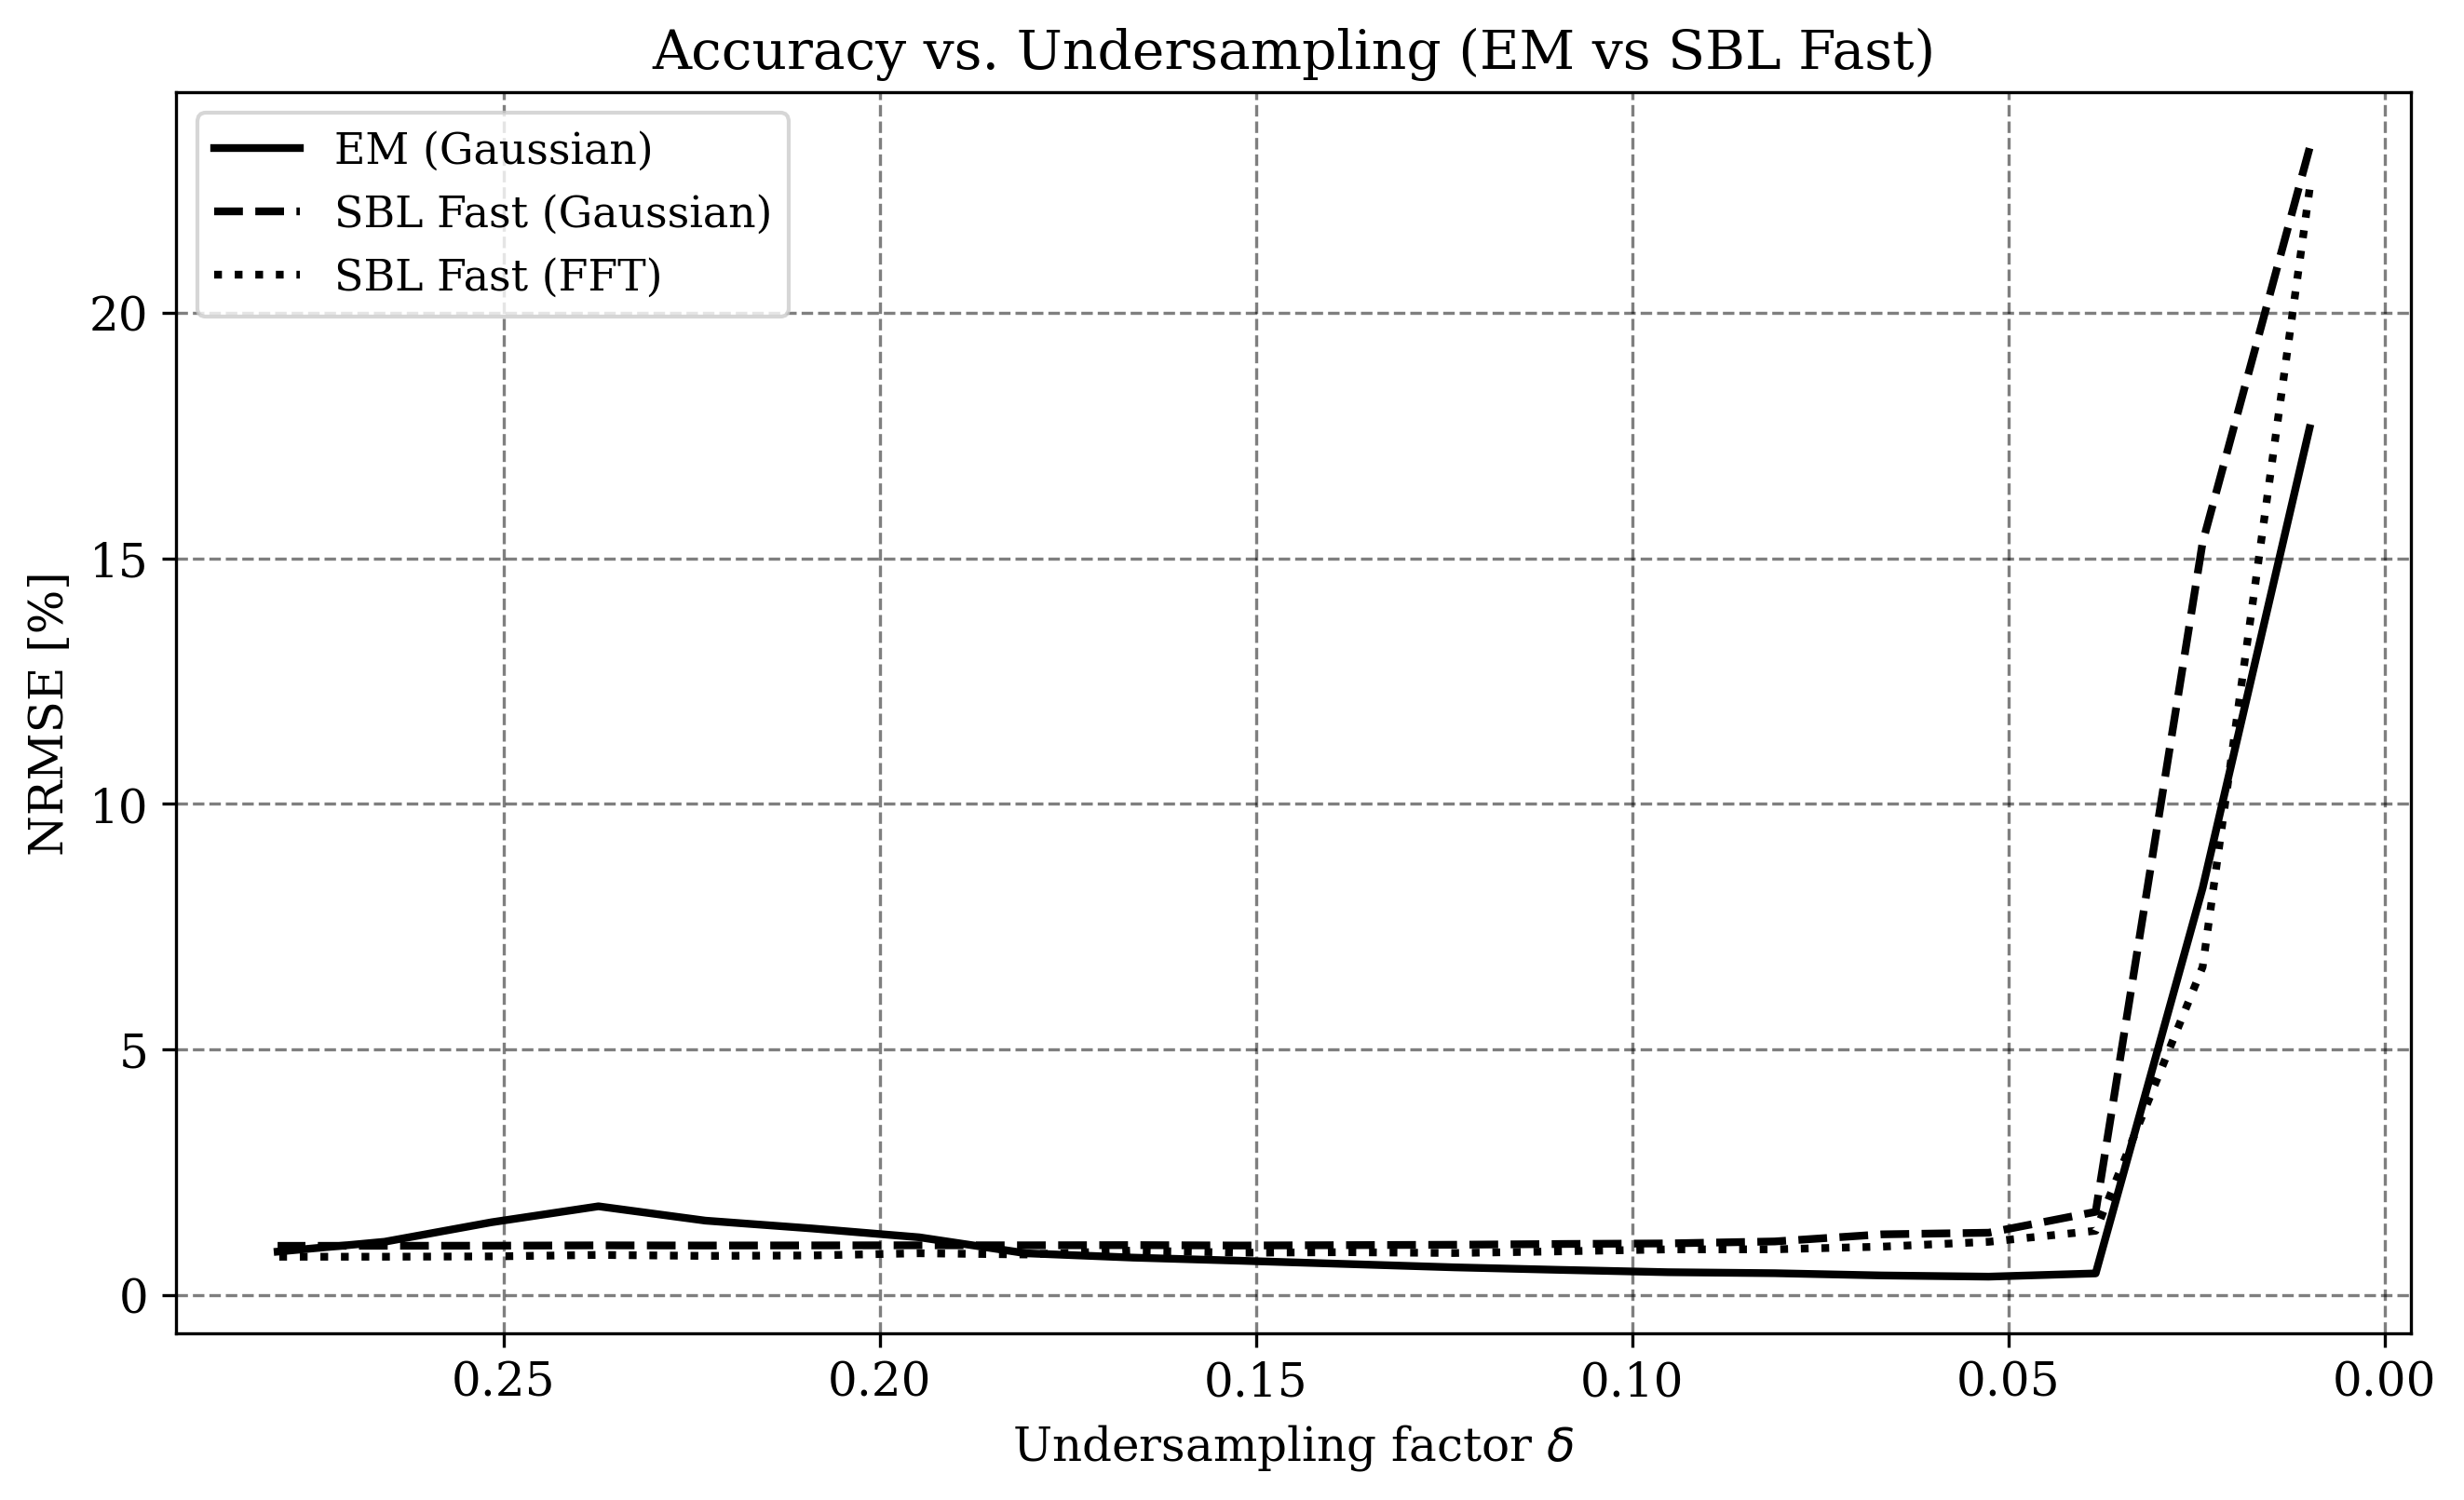
\includegraphics[width=0.75\linewidth]{Figures/accuracy_vs_undersampling_EMvsSB_woEMFFT.png}
    \caption{Reconstruction accuracy (NRMSE) versus undersampling factor $\delta$. Tipping’s algorithm maintains consistent performance across Gaussian and complex systems, while EM (excluded here for instability) was restricted to Gaussian cases.}
    \label{fig:accuracy_vs_undersampling_EMSB}
\end{figure}

\begin{figure}[H]
    \centering
    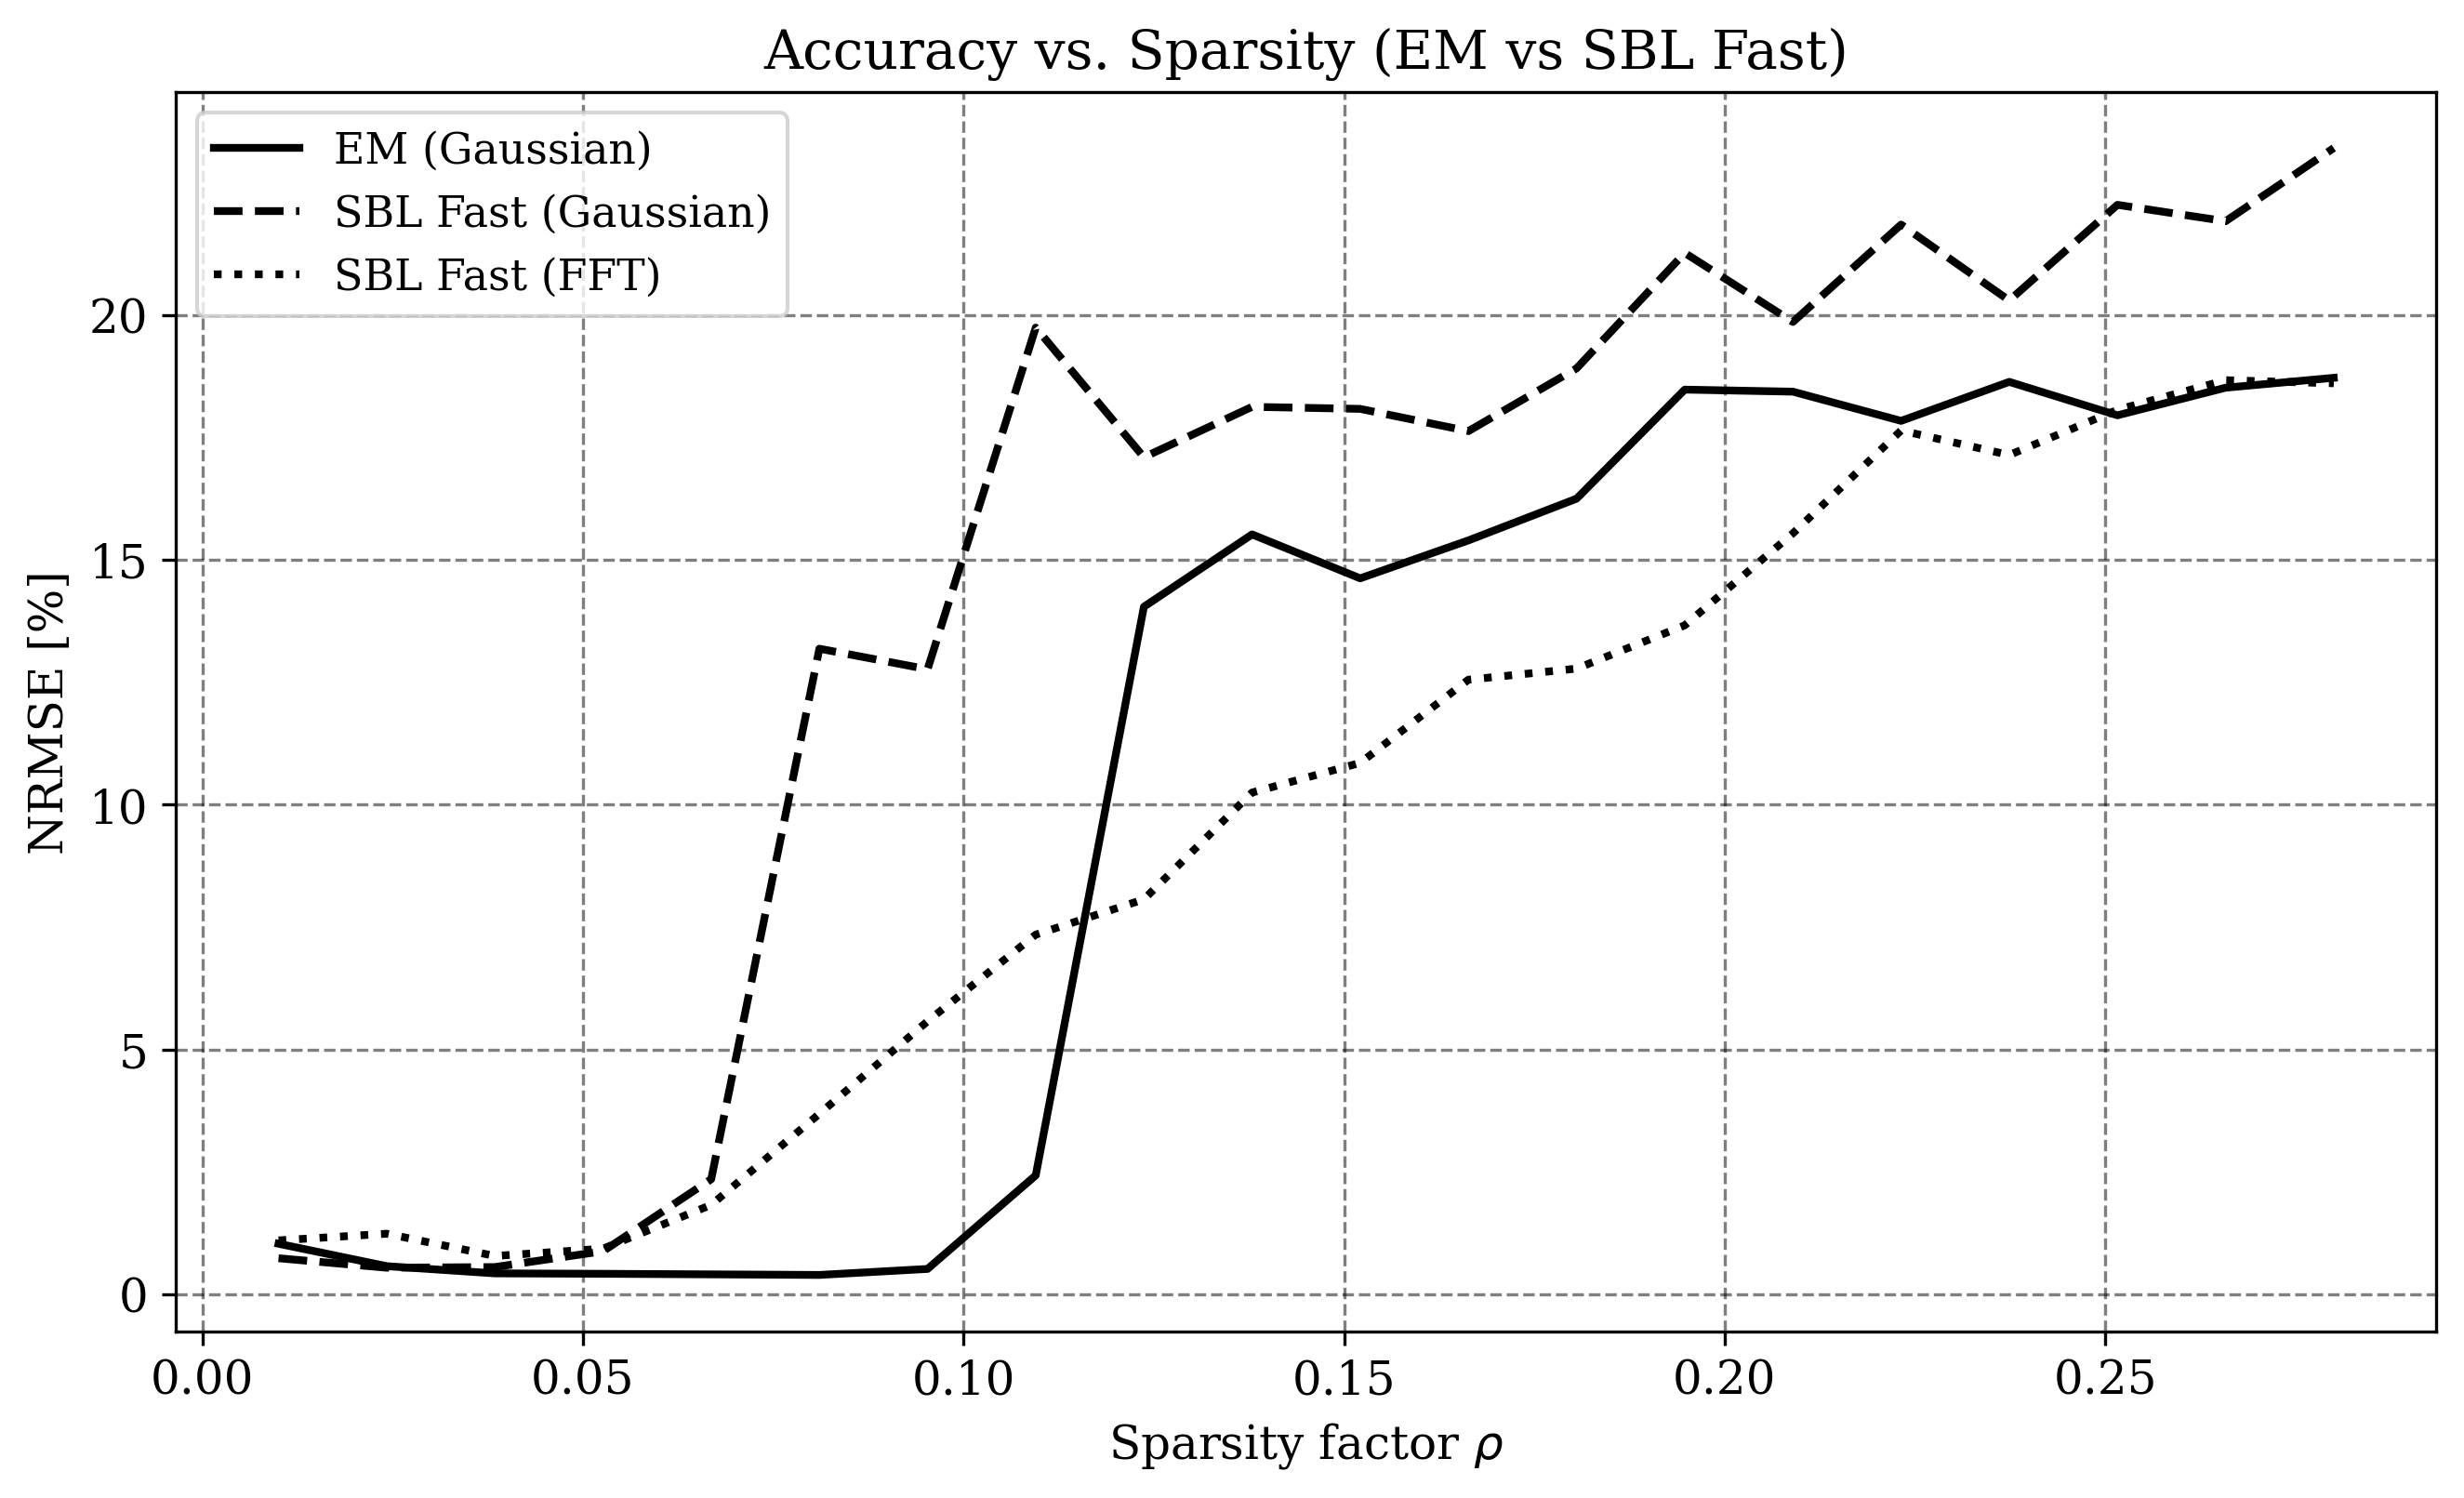
\includegraphics[width=0.75\linewidth]{Figures/accuracy_vs_sparsity_EMvsSB_woEMFFT.png}
    \caption{Reconstruction accuracy (NRMSE) versus ground-truth sparsity ratio $\rho$. Tipping’s method excels in complex systems, achieving lower NRMSE than in Gaussian cases—a reversal of EM’s behavior.}
    \label{fig:accuracy_vs_sparsity_EMSB}
\end{figure}

\subsection{Computational Efficiency}
Figure \ref{fig:runtimeSBl} compares the execution times of EM, CoFEM, and the Fast Marginal Likelihood algorithm under standardized conditions:
\begin{itemize}
\item Sparsity ratio $ \rho = 0.1 $
\item Noise variance $ \sigma^2 = 10^{-6} $
\item Convergence criterion $\frac{|\mathbf{t} - \Phi \boldsymbol{\mu}|_2}{|\mathbf{t}|_2} < 10^{-2}$
\end{itemize}


\begin{figure}[H]
    \centering
    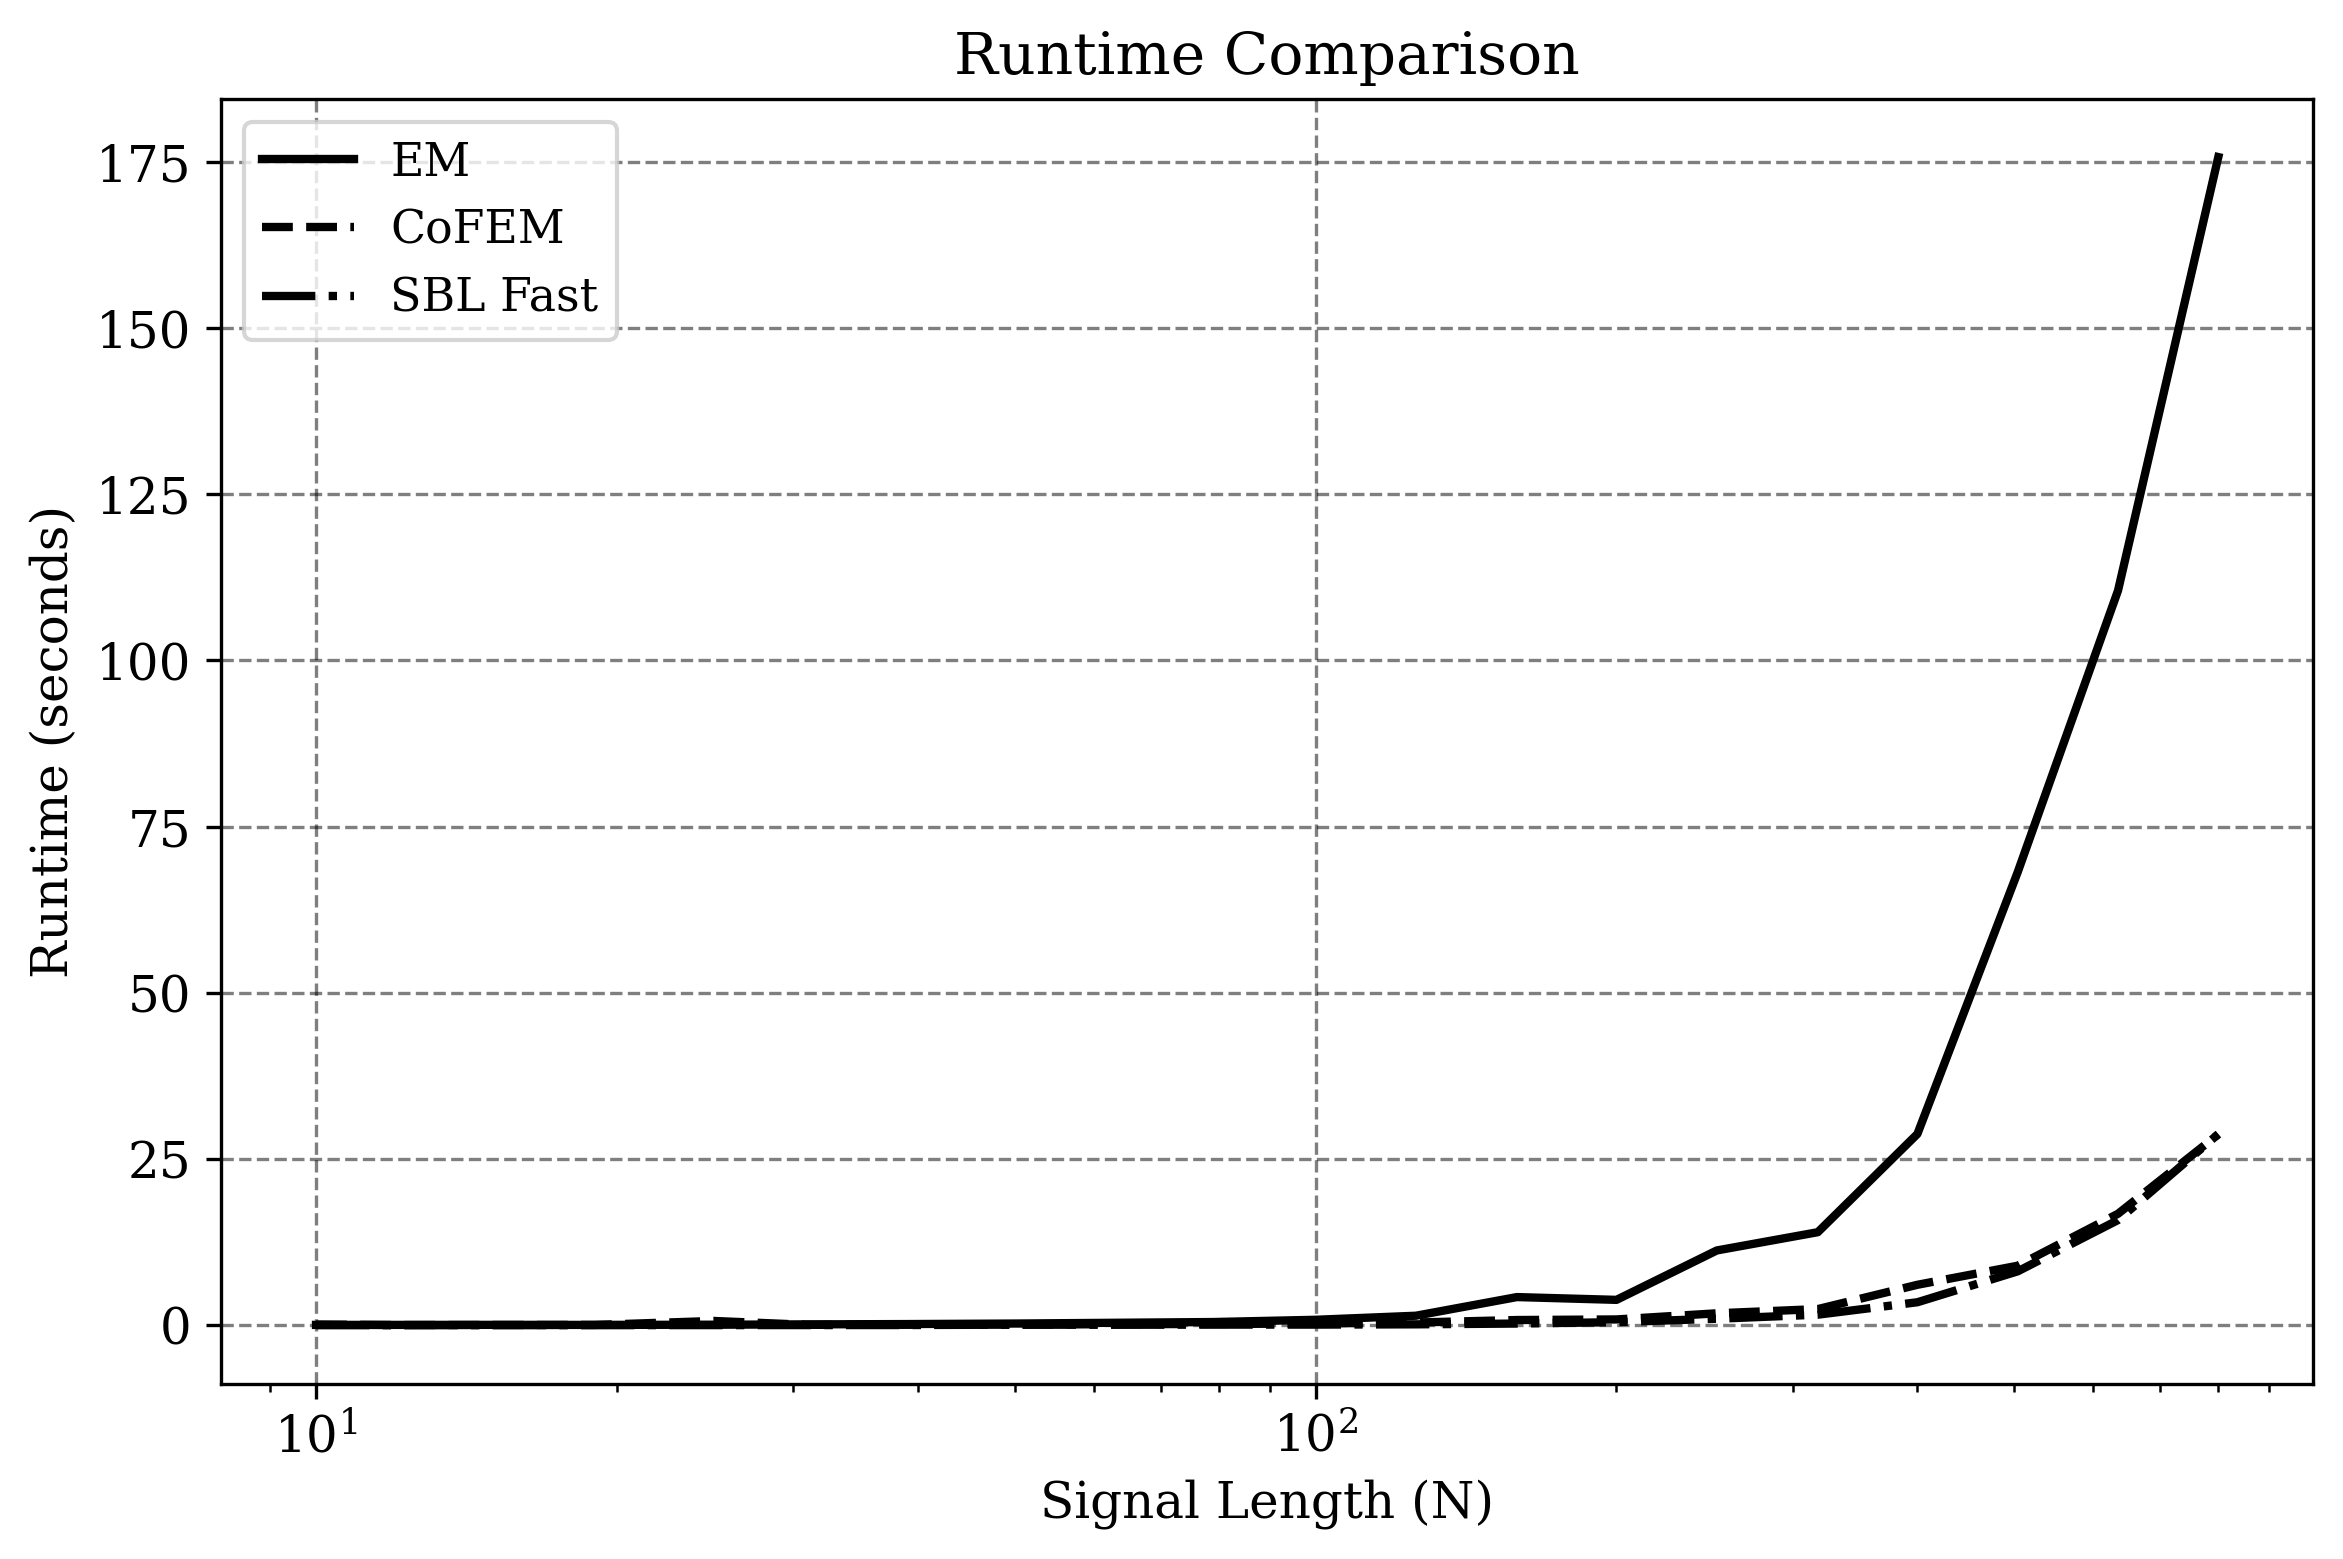
\includegraphics[width=0.75\linewidth]{Figures/runtime_comp_EMCoFEMSBL.png}
    \caption{Runtime versus measurement count $N$ for Gaussian dictionaries ($D=3N$). The Fast Marginal Likelihood algorithm exhibits the same computational efficiency as CoFEM and achieves significant speedups over EM, particularly at larger scales.}
    \label{fig:runtimeSBl}
\end{figure}

\subsection{Sparsity}
A critical distinction lies in how each algorithm enforces sparsity. Tipping’s method explicitly adds or prunes basis functions, yielding strictly sparse solutions. In contrast, EM gradually attenuates irrelevant weights toward near-zero values without exact truncation. Under low-noise conditions ($\sigma=0.01$), both methods successfully identify the true support while suppressing extraneous coefficients, as shown in Figures \ref{fig:weight01Gauss} and \ref{fig:weight01FFT}.
\begin{figure}[H]
    \centering
    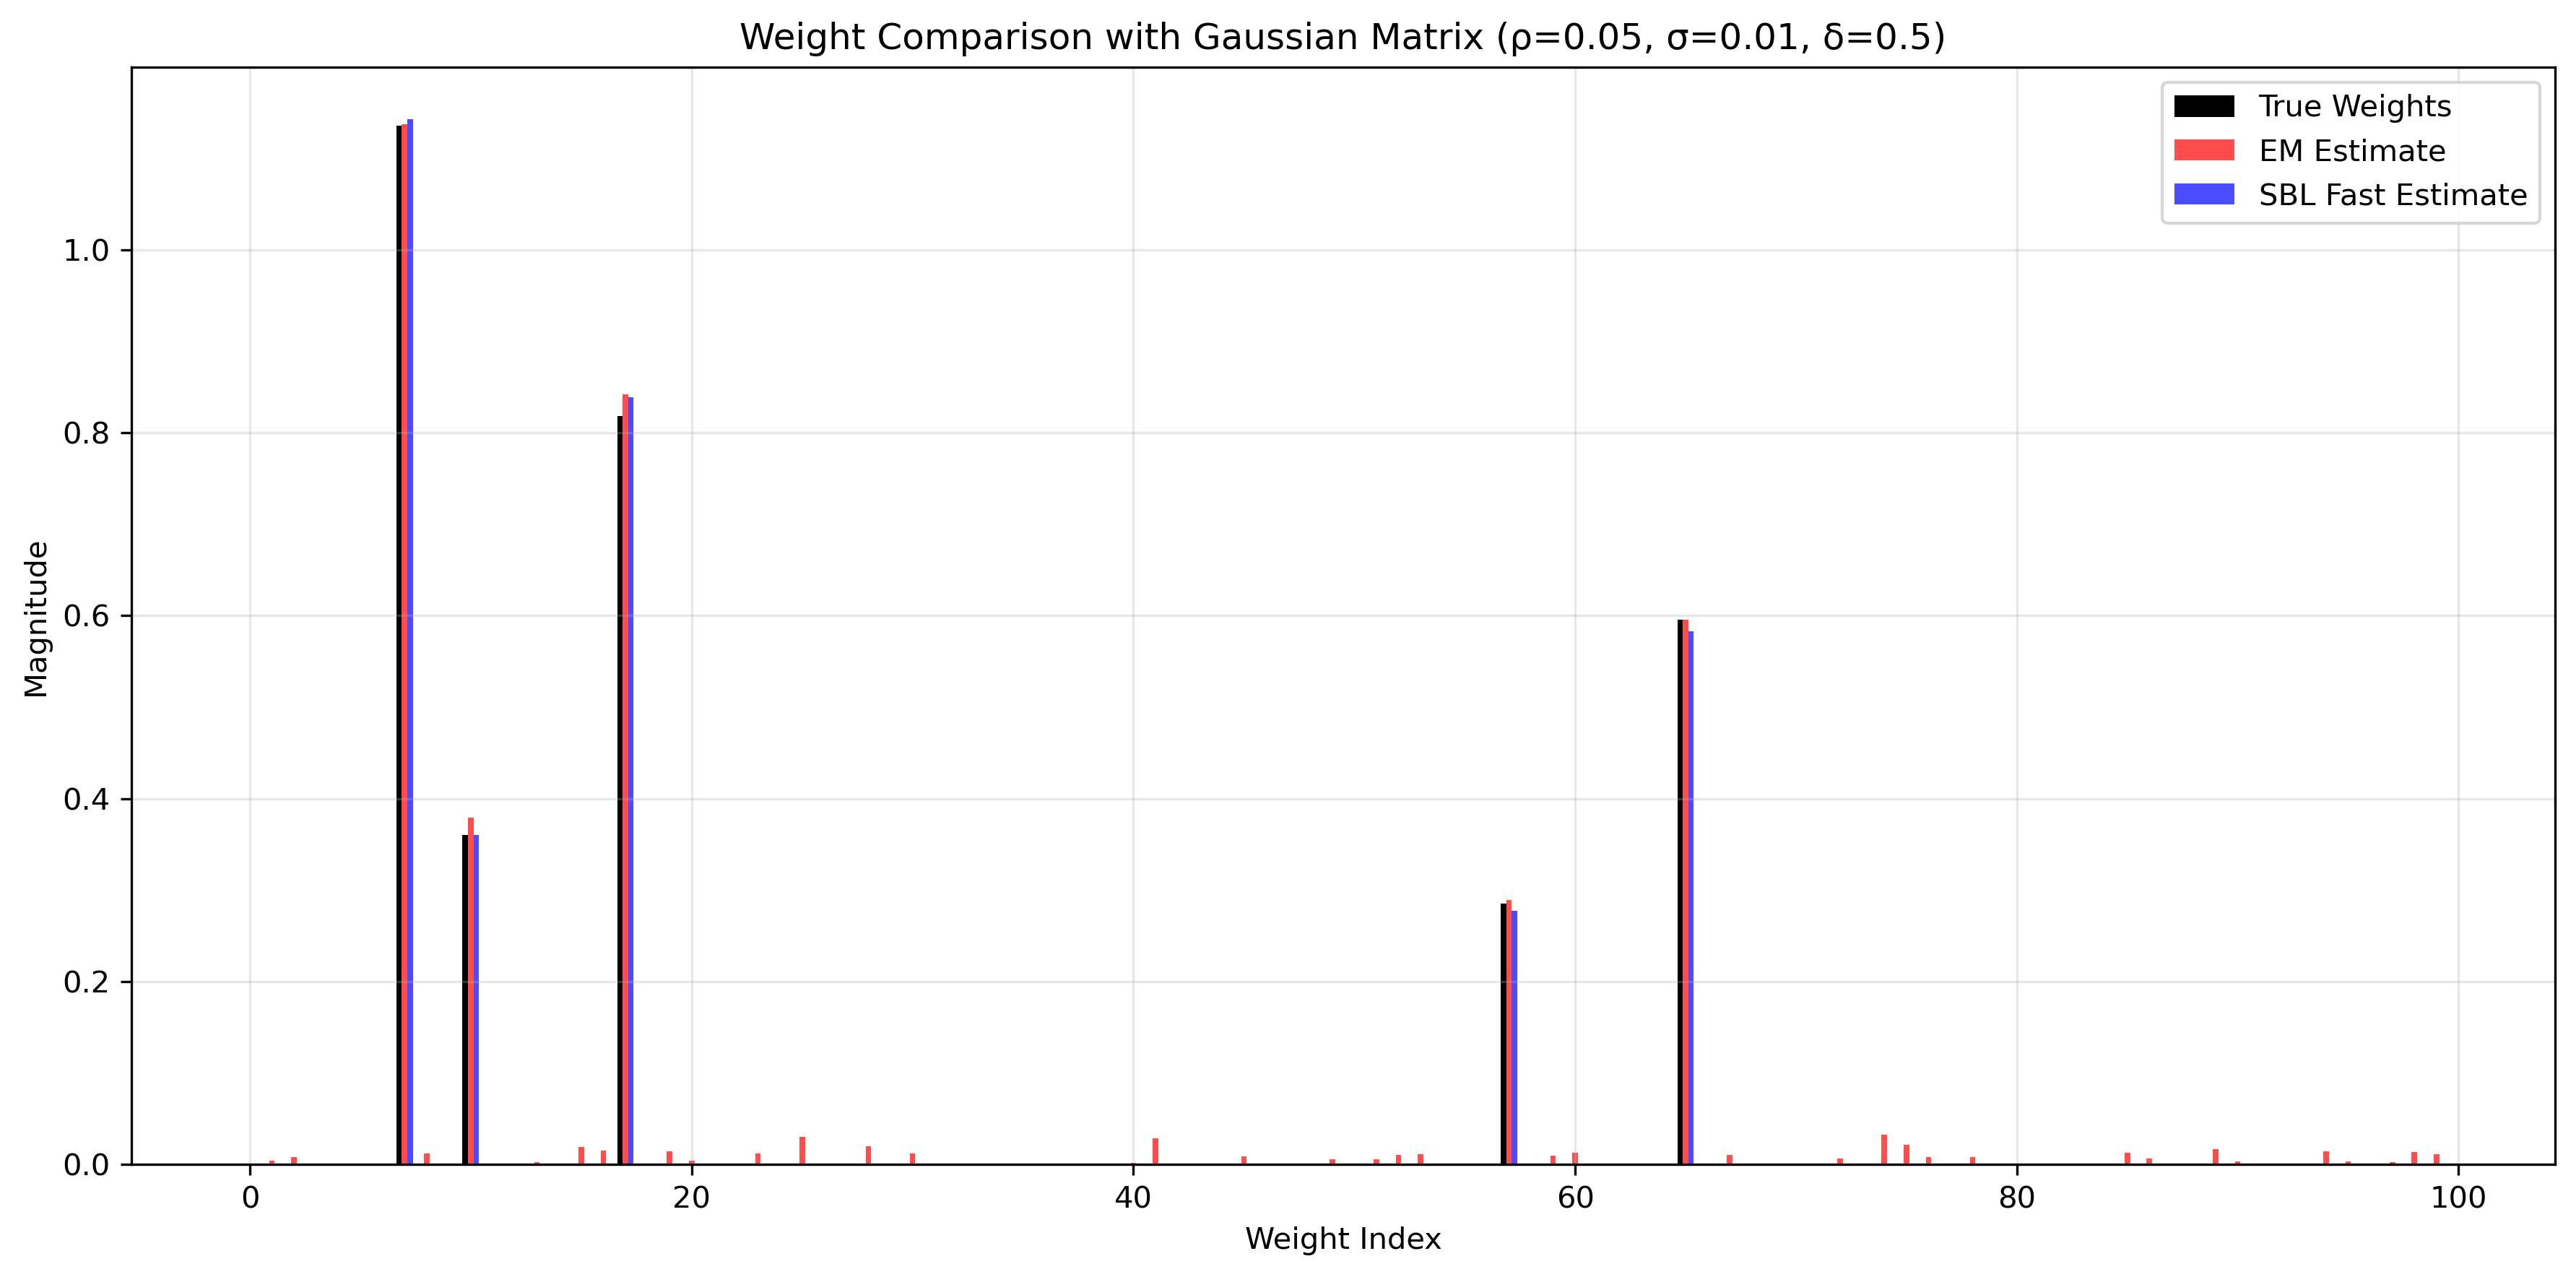
\includegraphics[width=0.75\linewidth]{Figures/weight_comparison_Gaussian_simga0.01.png}
    \caption{Weight magnitude comparisons (Gaussian dictionary, $\sigma=0.01$). Both algorithms recover the true support, though SBL produces strictly sparse estimates.}
    \label{fig:weight01Gauss}
\end{figure}
\begin{figure}[H]
    \centering
    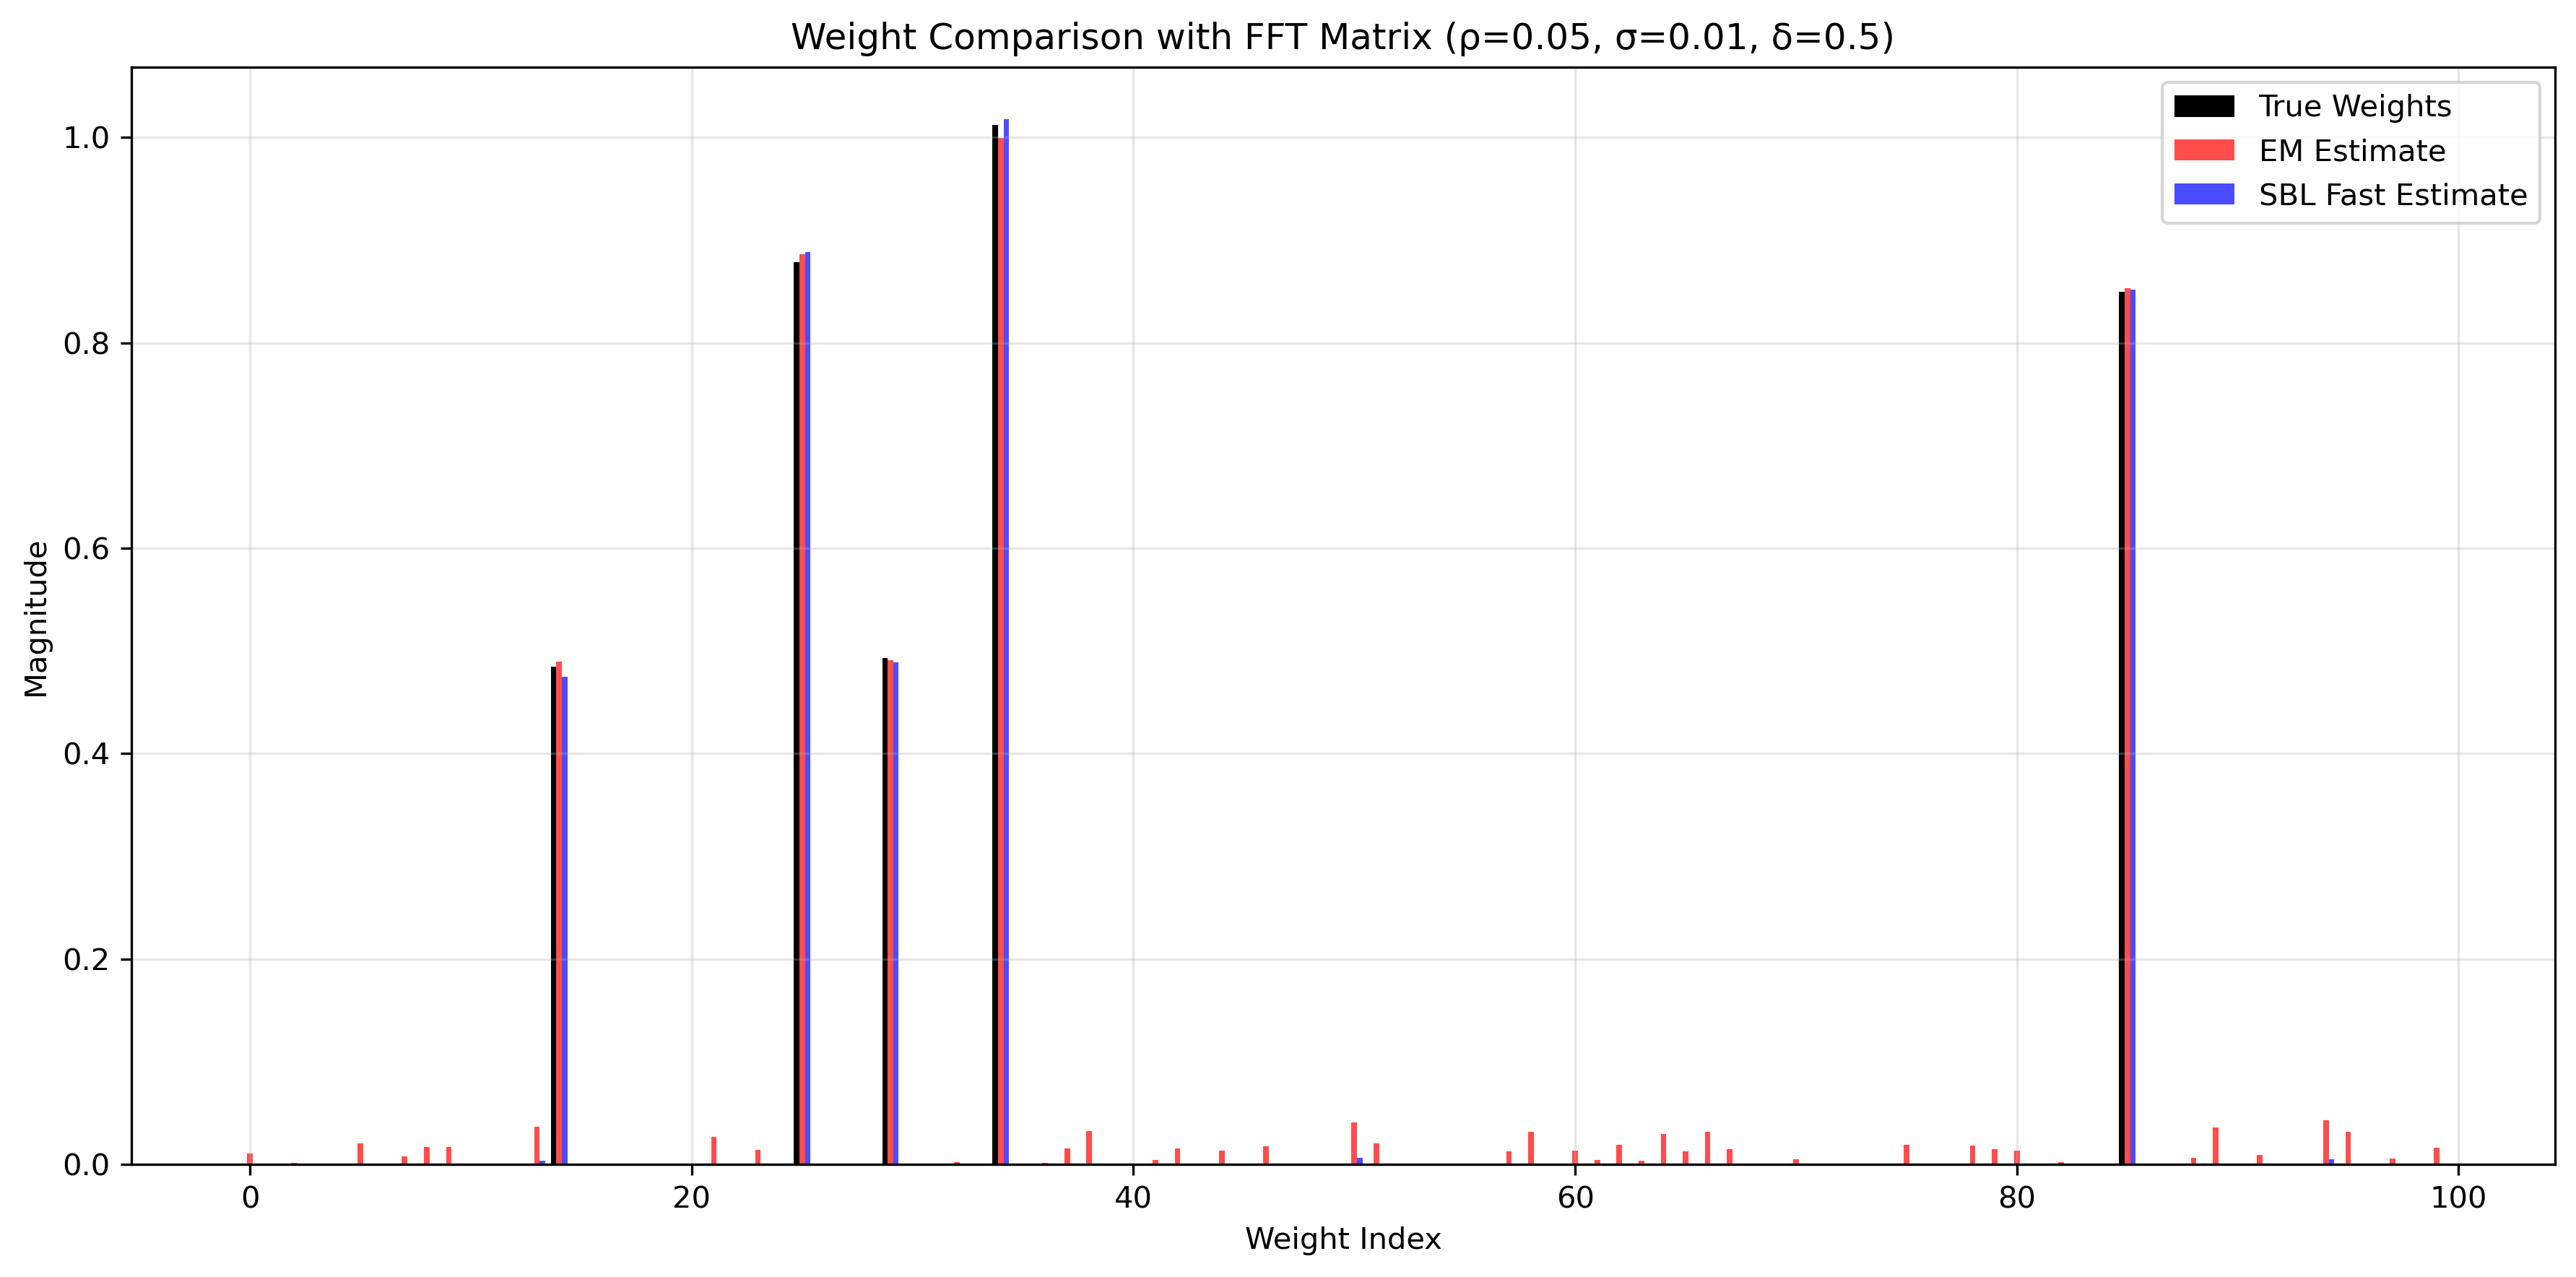
\includegraphics[width=0.75\linewidth]{Figures/weight_comparison_FFT_simga0.01.png}
    \caption{Weight magnitude comparisons (complex-valued dictionary, $\sigma=0.01$). SBL’s explicit basis selection enhances sparsity enforcement in Fourier-like systems.}
    \label{fig:weight01FFT}
\end{figure}

At higher noise levels ($\sigma=0.01$), Figures \ref{fig:weight001Gauss} and \ref{fig:weight001FFT} reveal comparable challenges: neither algorithm reliably identifies the true support, though SBL maintains stricter sparsity through its deletion mechanism.

\begin{figure}[H]
    \centering
    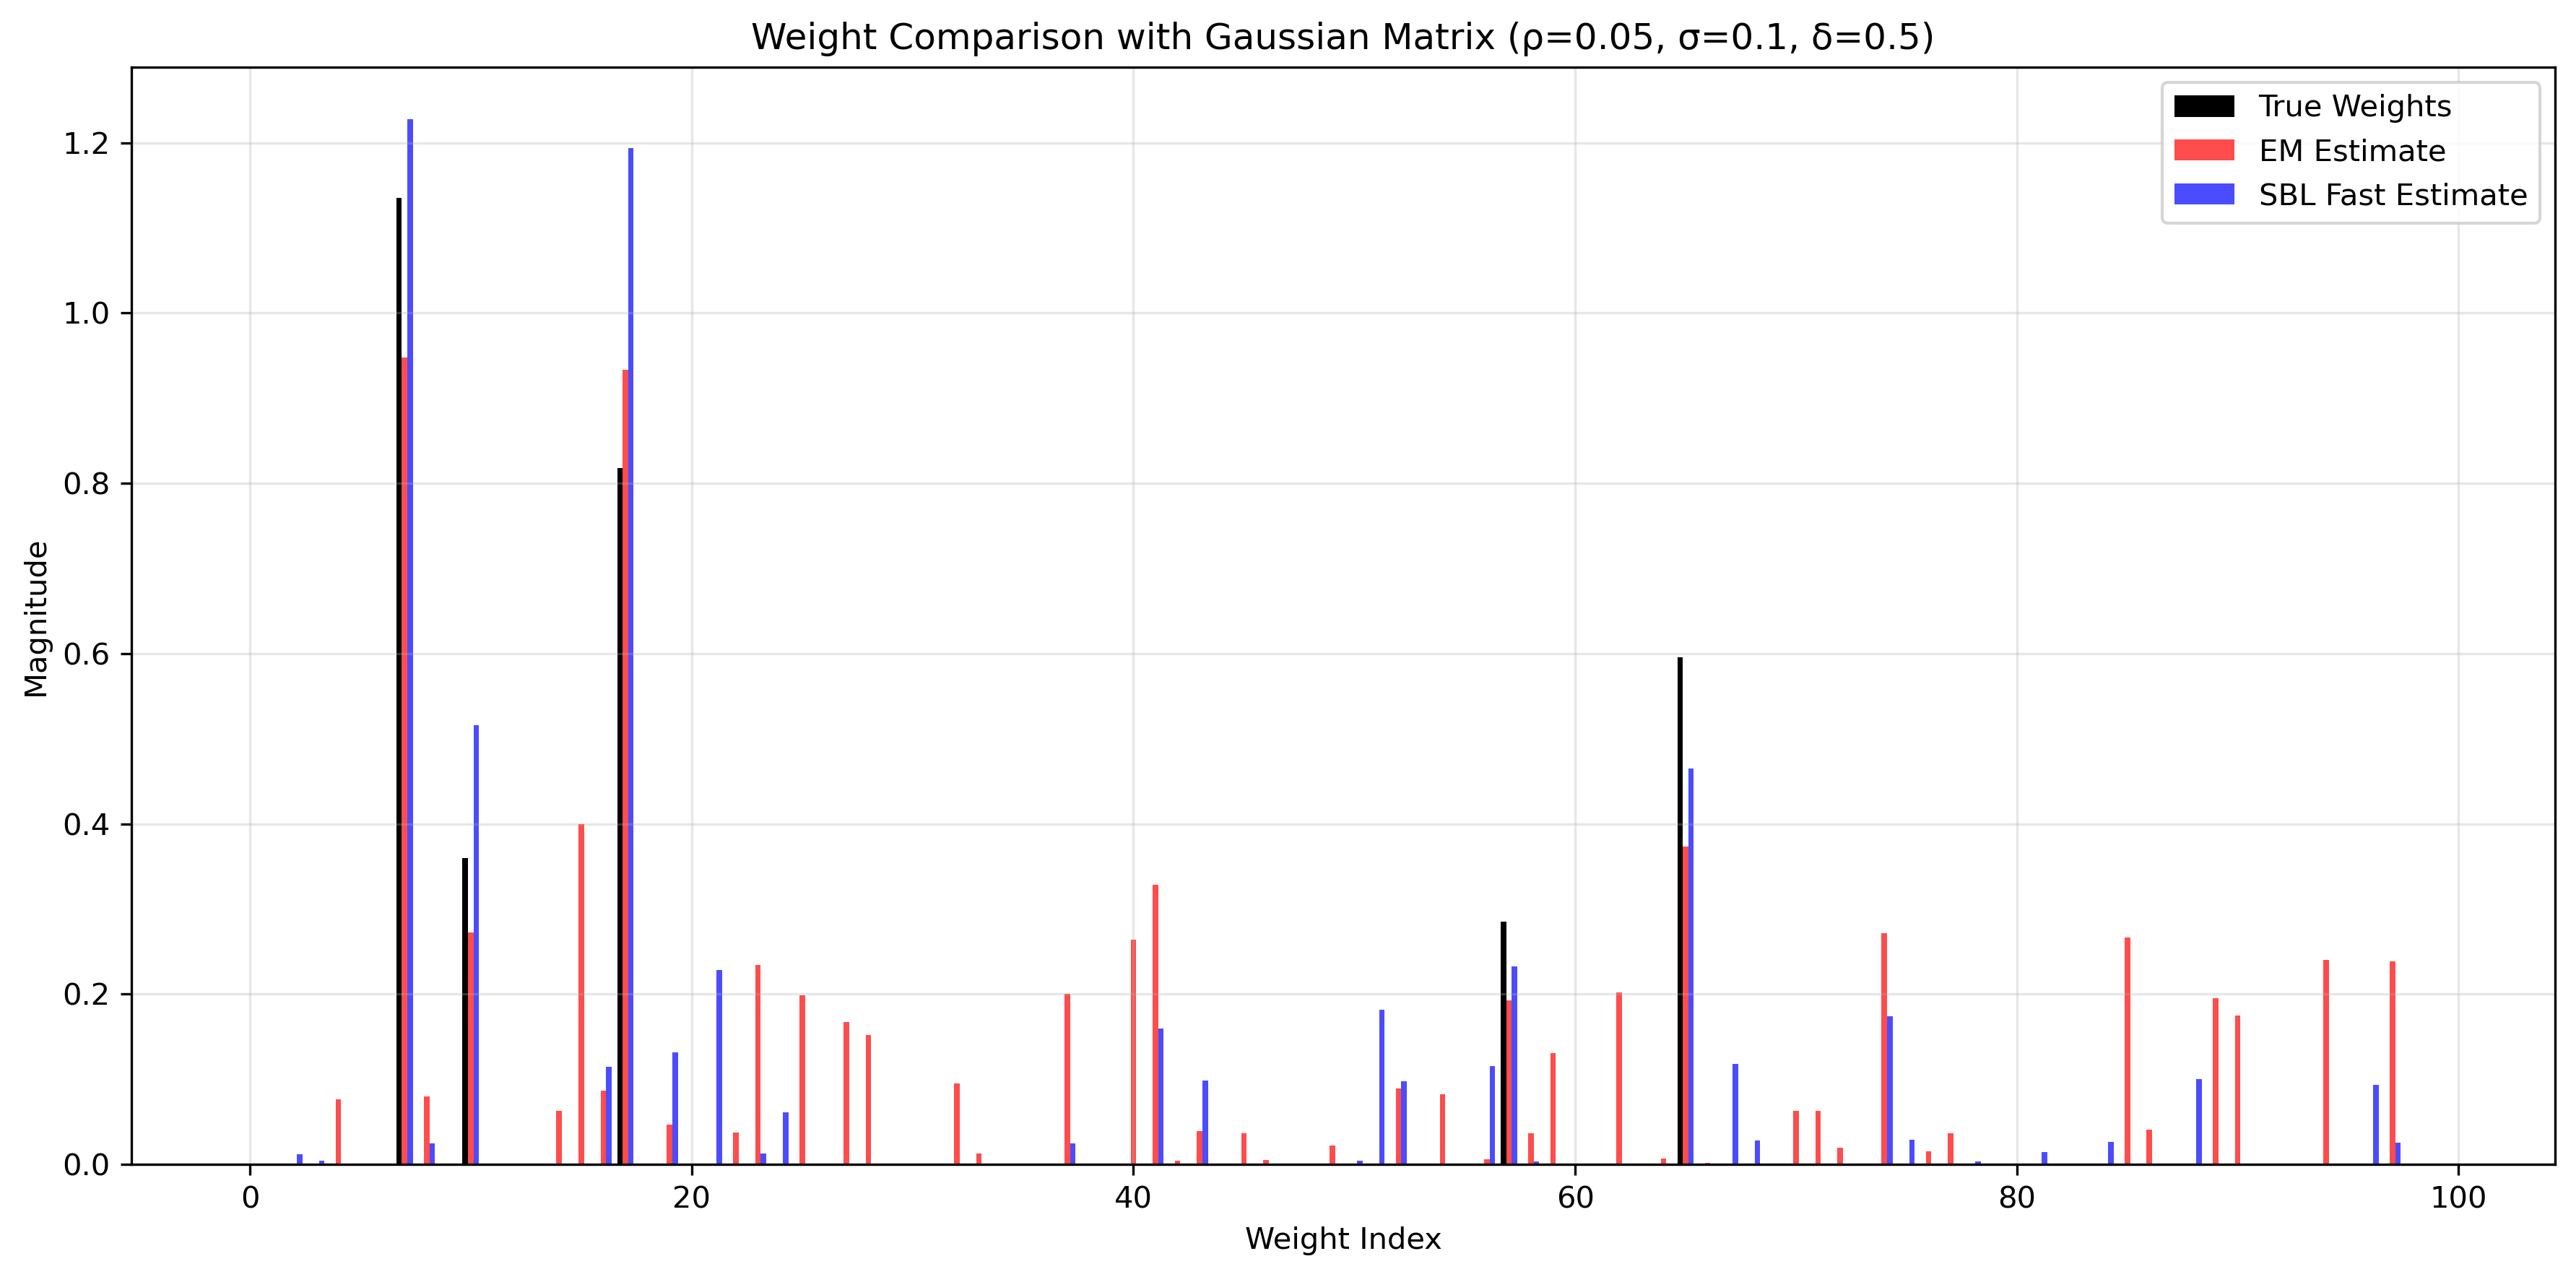
\includegraphics[width=0.75\linewidth]{Figures/weight_comparison_Gaussian_simga0.1.png}
    \caption{Weight estimates under moderate noise (Gaussian dictionary, $\sigma=0.01$). Both methods struggle with support recovery, though SBL avoids non-zero artifacts more effectively.}
    \label{fig:weight001Gauss}
\end{figure}
\begin{figure}[H]
    \centering
    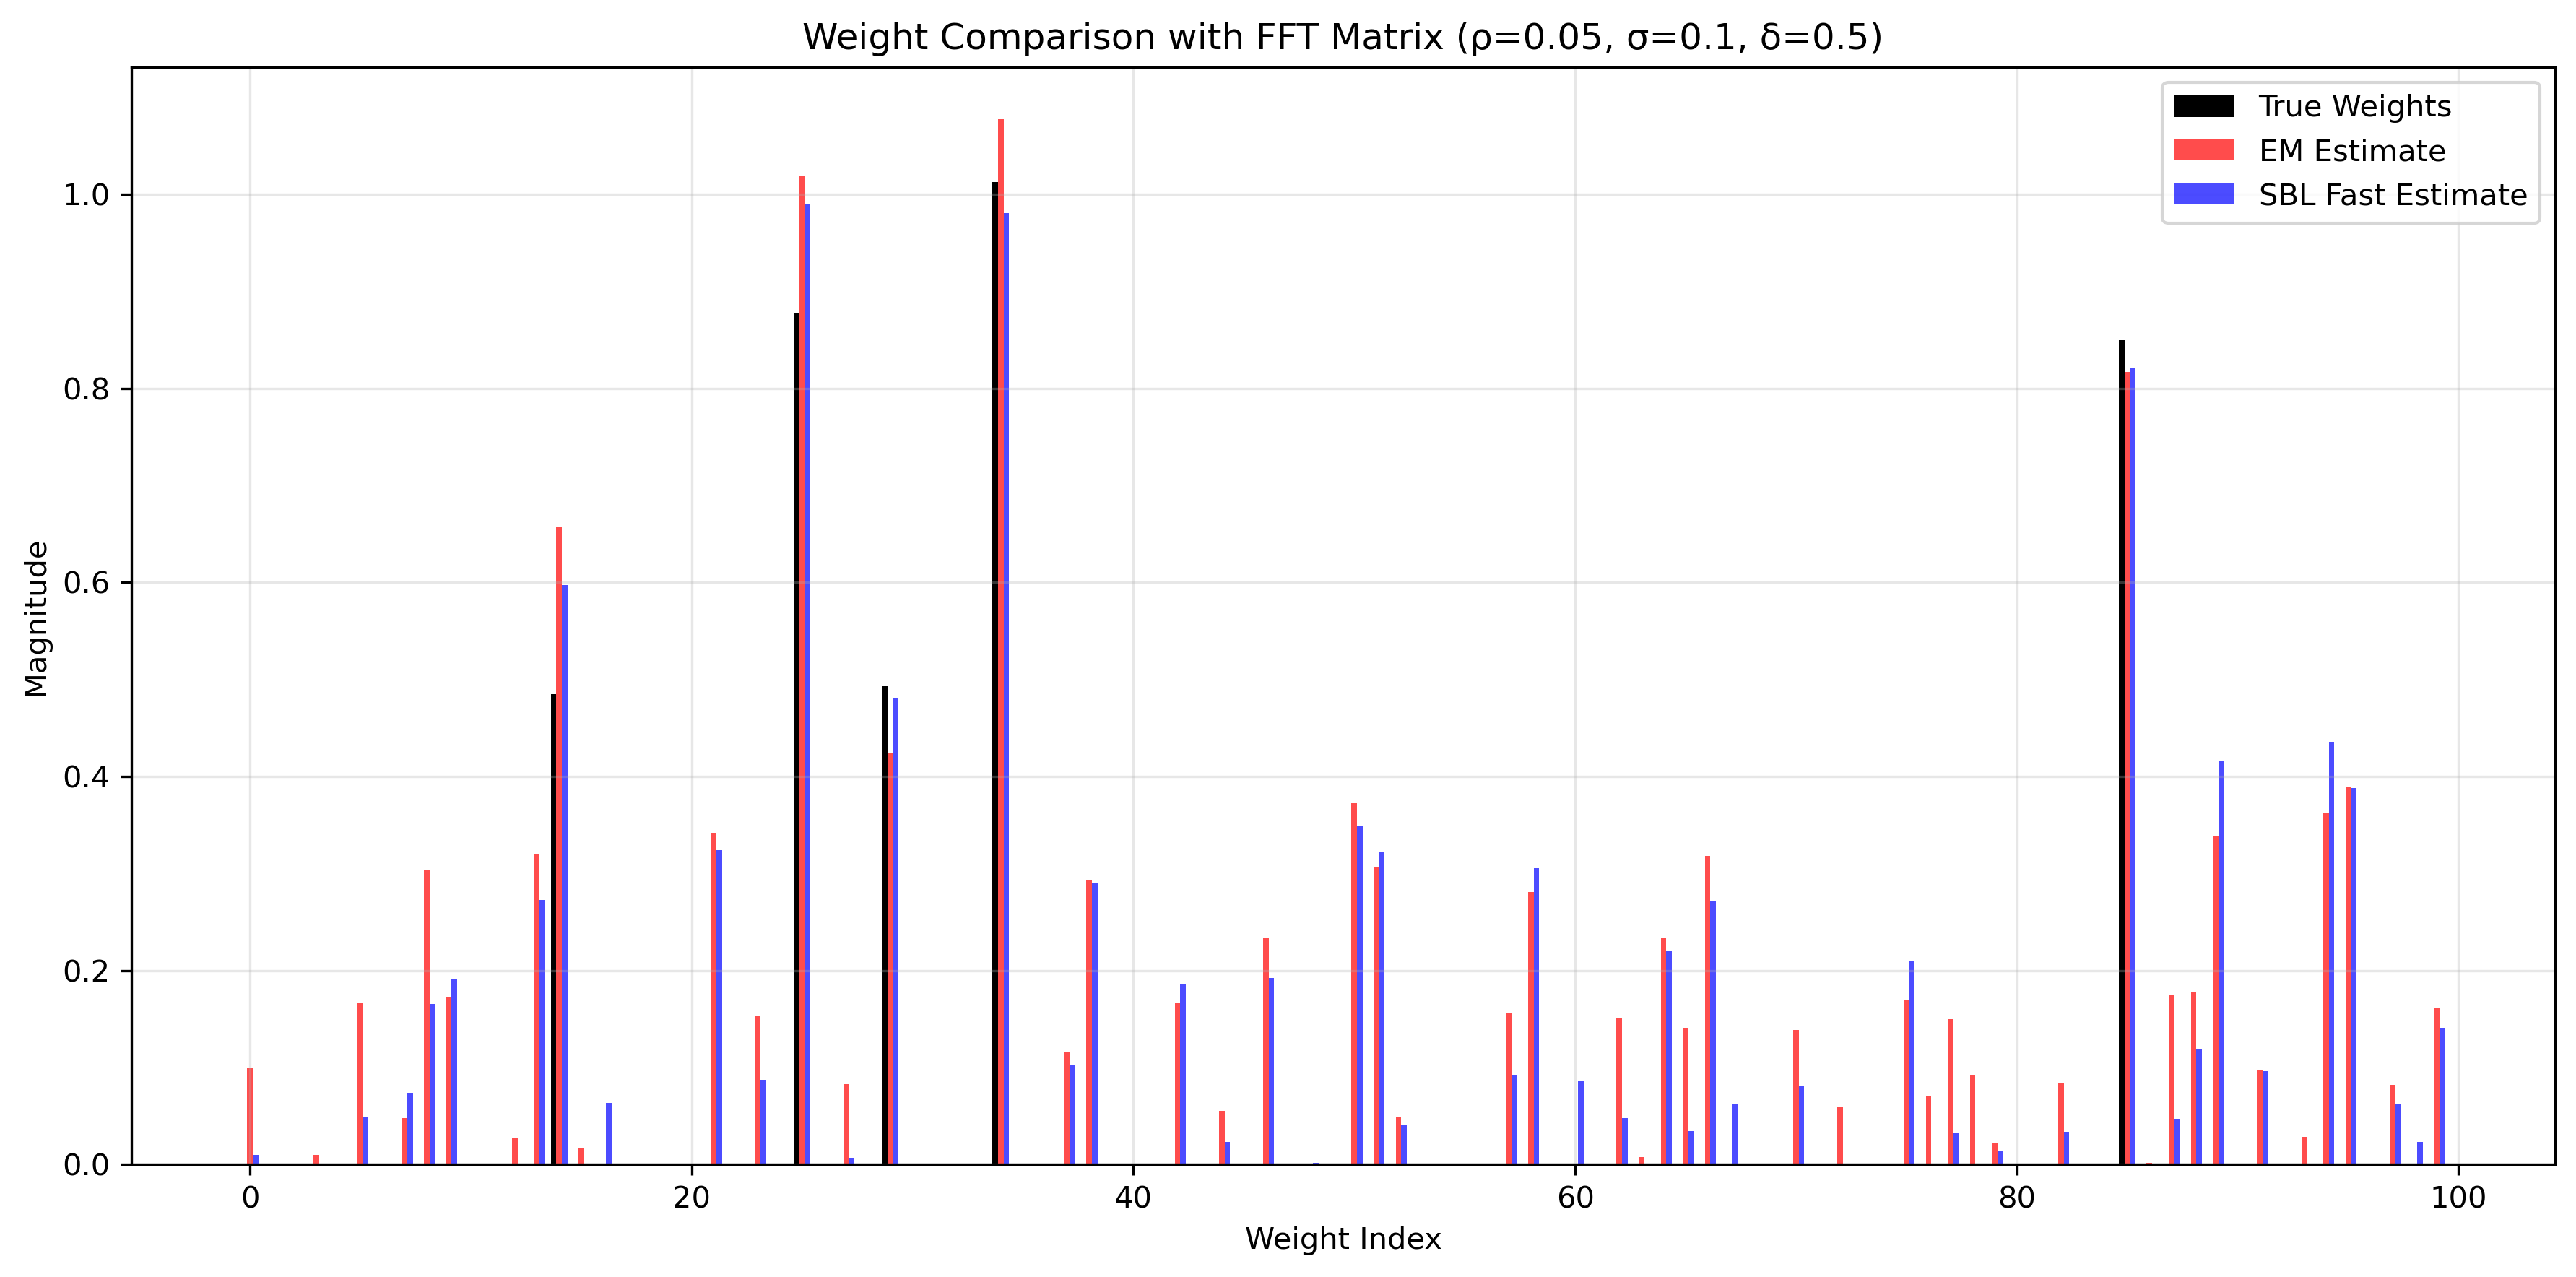
\includegraphics[width=0.75\linewidth]{Figures/weight_comparison_FFT_simga0.1.png}
    \caption{Weight estimates under moderate noise (complex-valued dictionary, $\sigma=0.01$). Both methods struggle with support recovery, though SBL avoids non-zero artifacts more effectively.}
    \label{fig:weight001FFT}
\end{figure}

\section{Spherical Near-Field Antenna Patterns}
\subsection{Spherical-Wave Expansion}

Spherical wave expansion (SWE) provides a mathematical framework for analyzing electromagnetic fields, particularly those radiated by antennas. By decomposing the electric field \(\mathbf{E}(r, \theta, \phi)\) into a sum of orthogonal spherical wave functions \(\mathbf{m}_{e,o_{mn}}\) and \(\mathbf{n}_{e,o_{mn}}\), SWE enables a systematic representation of the field in terms of outward-traveling waves. The expansion coefficients \(a_{e,o_{mn}}\) and \(b_{e,o_{mn}}\) are determined by projecting the tangential components of the field onto these basis functions, as shown in the integral expressions. This approach is especially useful for antenna characterization, near-field to far-field transformations, and scattering analysis, as it captures the field's angular and radial dependencies in a compact and physically meaningful way. The use of Hankel functions of the second kind ensures that only outward-propagating waves are considered, making SWE well-suited for problems involving radiation from finite sources. \citet{Ludwig1971NearfieldFT} presents how to derive the coefficients \(a_{e,o_{mn}}\) (TE waves) and \(b_{e,o_{mn}}\) (TM waves) in order to present the electric field like:
\begin{equation}
    \mathbf{E}(r,\theta,\phi)=-\sum_{m=-n}^n \sum_{n=1}^\infty a_{e,o_{mn}} \mathbf{m}_{e,o_{mn}} + b_{e,o_{mn}} \mathbf{n}_{e,o_{mn}}
\end{equation}
where the harmonic functions are defined as
\begin{equation}
    \begin{split}
        \mathbf{m}_{e,o_{mn}} =& \mp z_n(kr) \frac{m P_n^m(\cos \theta)}{\sin \theta} \stackanchor{$\sin$}{$\cos$} m \phi \, \boldsymbol{\hat{\theta}} \\
        &- z_n(kr) \frac{\partial}{\partial \theta} P_n^m(\cos \theta)\stackanchor{$\cos$}{$\sin$}m\phi \boldsymbol{\hat{\phi}}\\
        \mathbf{n}_{e,o_{mn}} =& n(n+1) \frac{z_n(kr)}{kr} P_n^m(\cos \theta)\stackanchor{$\sin$}{$\cos$} m \phi \boldsymbol{\hat{r}} \\
        &+ \frac{1}{kr} \frac{\partial}{\partial r} \left[ r z_n(kr) \right] \frac{\partial}{\partial \theta} P_n^m(\cos \theta)\stackanchor{$\sin$}{$\cos$} m \phi \boldsymbol{\hat{\theta}} \\
        &\pm \frac{1}{k r} \frac{\partial}{\partial r} \left[r z_n(k r) \right] \frac{m P_n^m(\cos \theta)}{\sin \theta}\stackanchor{$\cos$}{$\sin$} m \phi \boldsymbol{\hat{\phi}}
    \end{split}
\end{equation}
where \(P_n^{|m|}(\cos \theta)\) is the associated Legendre function. The radial function \(z_n^{(c)}(kr)\) depend on the wave type \(c\) and are defined as:
\begin{equation}
    z_n^{(c)}(kr) = \begin{cases}
        j_n(kr) & , c = 1 \\
        n_n(kr) & , c = 2 \\
        h_n^{(1)}(kr) = j_n(kr) + i n_n(kr) & , c = 3 \\
        h_n^{(2)}(kr) = j_n(kr) - i n_n(kr) & , c = 4
    \end{cases}
\end{equation}
In this case the Hankel function of second kind (\(j_n-iy_n)\) is used as \(z_n\), since only outward travelling waves are considered and the sources are assumed to have finite extend. The coefficients \(a_{e,o_{mn}}\) and \(b_{e,o_{mn}}\) an be obtained by solving the following integrals:
\begin{equation}
    \begin{split}
        a_{e,0_{mn}} =& \frac{1}{\left[z_n(kr_1)\right]^2} \frac{2n+1}{\pi 2n (n+1)} \frac{(n-m)!}{(n+m)!} \\
        &\cdot \int_0^{2\pi} \int_0^{\pi} -\mathbf{m}_{e,o_{mn}} \cdot \mathbf{E}(r_1, \theta, \phi)_{\tan} \sin \theta \, d\theta \, d\phi\\
        b_{e,o_{mn}} = &\frac{1}{\left[(1/kr_1)(\partial/\partial r) [r_1 z_n(kr_1)]\right]^2} \frac{2n + 1}{\pi 2n (n+1)} \frac{(n - m)!}{(n + m)!}\\
        &\cdot \int_0^{2\pi} \int_0^{\pi} -\mathbf{n}_{e,o_{mn}} \cdot \mathbf{E}(r_1, \theta, \phi)_{\tan} \sin \theta \, d\theta \, d\phi
    \end{split}
    \label{eq:expansion}
\end{equation}
Initial trials applied the formulas from \citet{Ludwig1971NearfieldFT} to expand the field of a simulated dipole antenna into spherical wave coefficients \(a_{e,o_{mn}}\) and \(b_{e,o_{mn}}\). The reconstructed field, derived from these coefficients, exhibited identical spatial patterns to the original field in 3D visualizations, but the magnitude scaling was inconsistent. Despite extensive literature review, the discrepancy remained unresolved. These coefficients would have served as a critical reference for validating subsequent Sparse Bayesian Learning results.


\subsection{SBL for Near Field Patterns}
\citet{Hofmann2019minimum} showed that the near-field of an antenna can be characterized with a minimum number of measurements under the assumption of sparsity in the spherical harmonics domain. The approach is based on expressing the near-field \(\mathbf{E}(r,\theta,\phi)\) as a linear combination of spherical vector wave functions \(\mathbf{h}_{smn}^{(4)}\). The theoretical framework is described in detail in \citet{hansen1988spherical}. In the following sections, the notation of Hansen will be used. The near-field is expressed as:

In this notation, \(s=1\) corresponds to \(\mathbf{n}\)-vector functions and \(s=2\) to the \(\mathbf{m}\)-vector functions. The use of even \(e\) and odd \(o\) modes is omitted by replacing \(\sin\) and \(\cos\) with complex exponential functions, reducing four real functions to two complex ones. The normalization is also modified. However, this notation is less common, and no explicit formulas for expansion via integration were found. Attempts to derive them independently were unsuccessful, resulting in incorrect magnitudes in the reconstructed field. Despite this, the compactness of the notation made it preferable for Sparse Bayesian Learning (SBL).
\begin{equation}
    \label{eq:hansenEfield}
    \mathbf{E}(r,\theta,\phi) = \frac{k}{\sqrt{\eta}}\sum_{c=3}^4\sum_{s=1}^2 \sum_{n=1}^\infty \sum_{m=-n}^m Q_{smn}^{(c)} \mathbf{F}_{smn}^{(c)}(r,\theta,\phi).
\end{equation}
\(\mathbf{E}(r,\theta,\phi)\) will correspond to \(\mathbf{t}\) in the SBL framework. Analogously, the spherical vector wave functions \(\mathbf{F}_{smn}^{(c)}(r,\theta,\phi)\) will be denoted as \(\Phi\) and \(Q_{smn}^{(c)}\) as \(\mathbf{w}\).

\(Q_{smn}^{(c)}\) are called the wave coefficients and are the unknowns to be estimated. \(\eta\) is the specific admittance and defined as \(\sqrt{\epsilon/\mu}\). \(c = 1\) and \(c = 2\) indicate standing waves, while \(c = 3\) represents an outward travelling wave, and \(c = 4\) an inward travelling wave. Since we regard only antennas in transmission mode in the abscence of refelction, only \(c=4\) will be regarded. \(s = 1\) denotes the m-function while \(s = 2\) gives the n-function. The spherical vector wave functions \(\mathbf{F}_{smn}^{(c)}(r,\theta,\phi)\) are defined as:
\begin{equation}
    \begin{split}
        \mathbf{F}_{1mn}^{(c)}(r,\theta,\phi) = &\frac{1}{\sqrt{2 \pi}} \frac{1}{\sqrt{n(n+1)}} \left( -\frac{m}{|m|} \right)^m \\
        &\Bigg\{ z_n^{(c)}(kr) \frac{i m \overline{P}_n^{|m|}(\cos \theta)}{\sin \theta} e^{i m \phi} \boldsymbol{\hat{\theta}} \\
        &- z_n^{(c)}(kr) \frac{\mathrm{d} \overline{P}_n^{|m|}(\cos \theta)}{\mathrm{d} \theta} e^{i m \phi} \boldsymbol{\hat{\phi}} \Bigg\} \\
        \mathbf{F}_{2mn}^{(c)}(r, \theta, \phi) = &\frac{1}{\sqrt{2\pi}} \frac{1}{\sqrt{n(n+1)}} \left( -\frac{m}{|m|} \right)^m \\
        &\Bigg\{ \frac{n(n+1)}{kr} z_n^{(c)}(kr) \bar{P}_n^{|m|}(\cos \theta) e^{im\phi} \boldsymbol{\hat{r}} \\
        &+ \frac{1}{kr} \frac{d}{d(kr)} \left( kr z_n^{(c)}(kr) \right) \frac{d \bar{P}_n^{|m|}(\cos \theta)}{d\theta} e^{im\phi} \boldsymbol{\hat{\theta}} \\
        &+ \frac{1}{kr} \frac{d}{d(kr)} \left( kr z_n^{(c)}(kr) \right) \frac{im \bar{P}_n^{|m|}(\cos \theta)}{\sin \theta} e^{im\phi} \boldsymbol{\hat{\phi}} \Bigg\}
    \end{split}
\end{equation}
where \(\bar{P}_n^{|m|}(\cos \theta)\) is the normalized associated Legendre function:
\begin{equation}
    \bar{P}_n^m(\cos \theta) = \sqrt{\frac{2n+1}{2} \frac{(n-m)!}{(n+m)!}} P_n^m(\cos \theta)
\end{equation}
The derivation of the normalized associated Legendre function can be expressed as:
\begin{equation}
    \begin{split}
        \frac{d \bar{P}_n^{|m|}(\cos \theta)}{d\theta} &= \frac{d \bar{P}_n^{|m|}(\cos \theta)}{d\cos \theta} \frac{d\cos \theta}{d\theta} \\
        &= -\sin\theta \sqrt{\frac{2n+1}{2} \frac{(n-m)!}{(n+m)!}} \frac{dP_n^{|m|}(\cos \theta)}{d\cos \theta}
    \end{split}
\end{equation}
The radial function \(z_n^{(c)}(kr)\) depend on the wave type \(c\) and are defined as:
\begin{equation}
    z_n^{(c)}(kr) = \begin{cases}
        j_n(kr) & , c = 1 \\
        n_n(kr) & , c = 2 \\
        h_n^{(1)}(kr) = j_n(kr) + i n_n(kr) & , c = 3 \\
        h_n^{(2)}(kr) = j_n(kr) - i n_n(kr) & , c = 4
    \end{cases}
\end{equation}

\subsection{Implementation}
In the SBL framework, the spherical harmonics domain is embedded by representing the measured electromagnetic field as a linear combination of spherical vector wave functions, which serve as the basis functions. The measurement matrix $\Phi$ (or $F$ in the code) has dimensions $(N, D, 3)$, where $N$ is the number of spatial sampling points (each corresponding to a unique pair of angles $(\theta, \phi)$), $D$ is the total number of spherical harmonics modes (indexed by $(n, m, s)$), and the third dimension corresponds to the three Spherical field components (e.g., $E_r$, $E_\theta$, $E_\phi$). The measurement vector $\mathbf{t}$ is initially a matrix of shape $(N, 3)$, containing the three field components at each spatial point. To apply the SBL algorithm, which requires a standard linear model with scalar-valued entries, both $\Phi$ and $\mathbf{t}$ are reshaped: $\Phi$ is transformed to a matrix of shape $(3N, D)$ by stacking the field components for all points, and $\mathbf{t}$ is flattened to a vector of length $3N$. This allows the vector-valued measurement problem to be cast as a standard SBL problem, where the physical structure of the spherical harmonics expansion is preserved in the dictionary and the mapping between physical and matrix dimensions is explicit.

\subsection{Antenna Simulation}

\subsection{Antenna Simulation}

To validate the SBL-based near-field reconstruction approach described above, a set of synthetic antenna measurements was generated using MATLAB's Antenna Toolbox. Initially, an attempt was made to simulate more complex antenna structures in CST Microwave Studio. However, due to limitations in the student version of CST, specifically the lack of support for exporting radiation patterns in spherical coordinates, this path was not viable for generating high-resolution spherical near-field data.

An alternative approach was adopted by modeling simple canonical antennas—specifically, a half-wave dipole and a loop antenna—operating at 2.4 GHz using MATLAB’s built-in functions. These provide well-defined and analytically tractable radiation characteristics, making them ideal for testing and validating reconstruction algorithms. The simulated electric field patterns were exported in spherical coordinates $(r, \theta, \phi)$, with a resolution of $1^\circ$ in both the polar ($\theta$) and azimuthal ($\phi$) directions.

Two distinct radial distances were considered for the field evaluation:
\begin{itemize}
    \item $r = 0.5\lambda$: representing the reactive near-field region.
    \item $r = 5\lambda$: approximating the radiating far-field region.
\end{itemize}

This allowed for comparative analysis between near- and far-field reconstructions, as well as verification of the method’s ability to capture the transition from near- to far-field behavior. The field components $E_r$, $E_\theta$, and $E_\phi$ were sampled on a uniform spherical grid at each radius, forming the measurement vector $\mathbf{t}$ used in the SBL framework. 

The results can be seen in figure \ref{fig:dipole_rad}.
\begin{figure}[H]
    \centering
    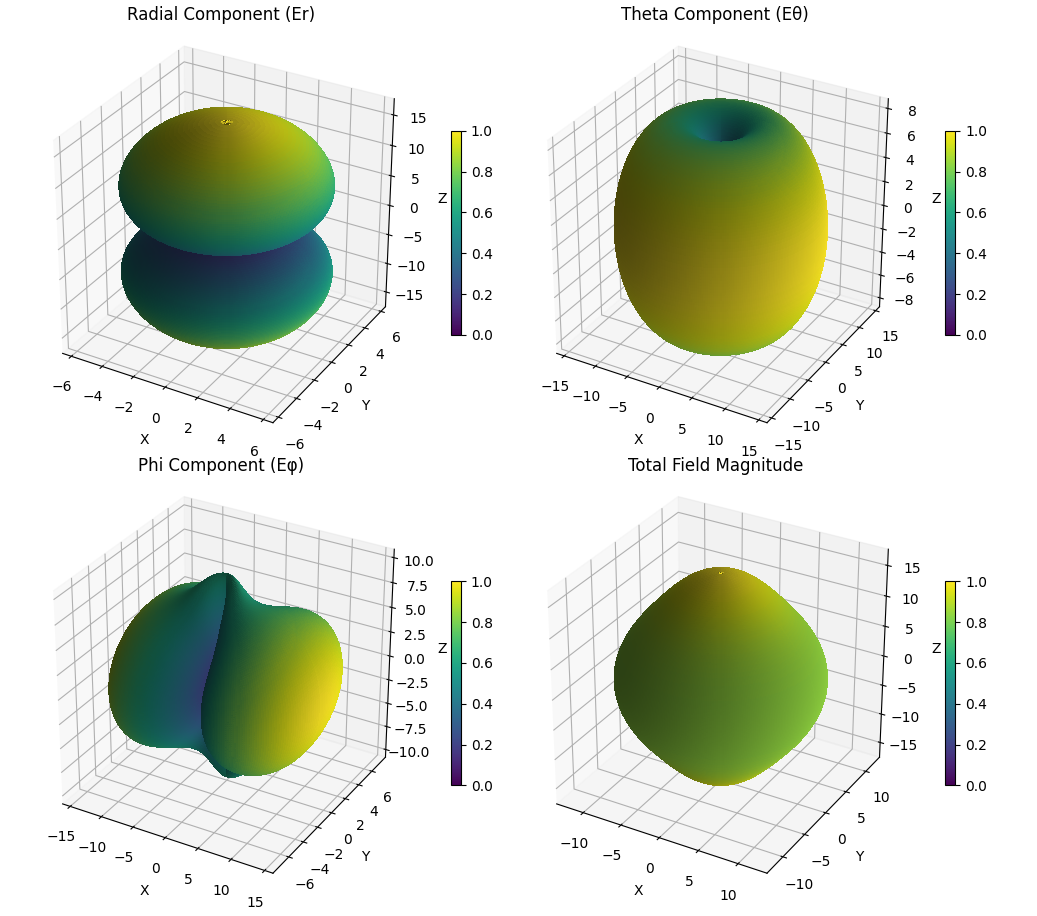
\includegraphics[width=0.75\linewidth]{Figures/Dipol_radiation.png}
    \caption{The magnitude of the farfield radiation pattern of the dipole antenna.}
    \label{fig:dipole_rad}
\end{figure}


\subsection{Far-Field Pattern Expansion and Reconstruction}

Initial experiments focused on the expansion of the simulated far-field radiation patterns into spherical vector wave harmonics, followed by their reconstruction using the derived coefficients. The electric field data obtained from MATLAB Antenna Toolbox at a radial distance of $r = 5\lambda$ (representing the far-field region) was used for this purpose.

The measurement matrix $\Phi$ (denoted as $F$ in implementation) was constructed based on the theoretical expressions of the spherical vector wave functions $\mathbf{F}_{smn}^{(c)}$, evaluated at the corresponding wavenumber $k$ and radius $r$. Subsequently, the wave coefficients $Q_{smn}^{(3)}$—corresponding to outward-propagating waves—were estimated using the Fast Marginal Likelihood Maximization algorithm.

To assess the accuracy of the expansion and reconstruction process, the original field $\mathbf{E}_{\text{org}}$ was reconstructed via $\mathbf{E}_{\text{rec}} = \Phi \mathbf{w}$, where $\mathbf{w}$ represents the estimated coefficient vector. The relative reconstruction error was quantified using the normalized mean squared error (MSE):
\[
\text{MSE}_{\text{rel}} = \frac{\|\mathbf{E}_{\text{rec}} - \mathbf{E}_{\text{org}}\|}{\|\mathbf{E}_{\text{org}}\|}.
\]

These experiments were conducted using $N_{\text{modes}} = 25$, resulting in a total of $D = 2N_{\text{modes}}^2 + 4N_{\text{modes}} = 1350$ basis functions. The spatial resolution of the input field was systematically reduced by downsampling the angular sampling grid $(\theta, \phi)$ with a factor $k$, leading to a varying number of measurement points $N$. The ratio $\delta = N/D$ was used as an independent variable to evaluate the reconstruction performance under different undersampling conditions.

Figure \ref{fig:mse_ff} shows the relative MSE as a function of $\delta$ for both the dipole and loop antennas. Notably, even at $\delta=1$, where the number of measurements equals the number of unknowns, significant reconstruction errors are observed, particularly for the loop antenna. Ideally, a perfect reconstruction should be achievable in such a scenario, suggesting potential issues related to numerical inaccuracies, implementation flaws in the spherical vector wave functions $\mathbf{F}_{smn}^{(c)}$, or misinterpretations of the underlying electromagnetic theory.
\begin{figure}[H]
    \centering
    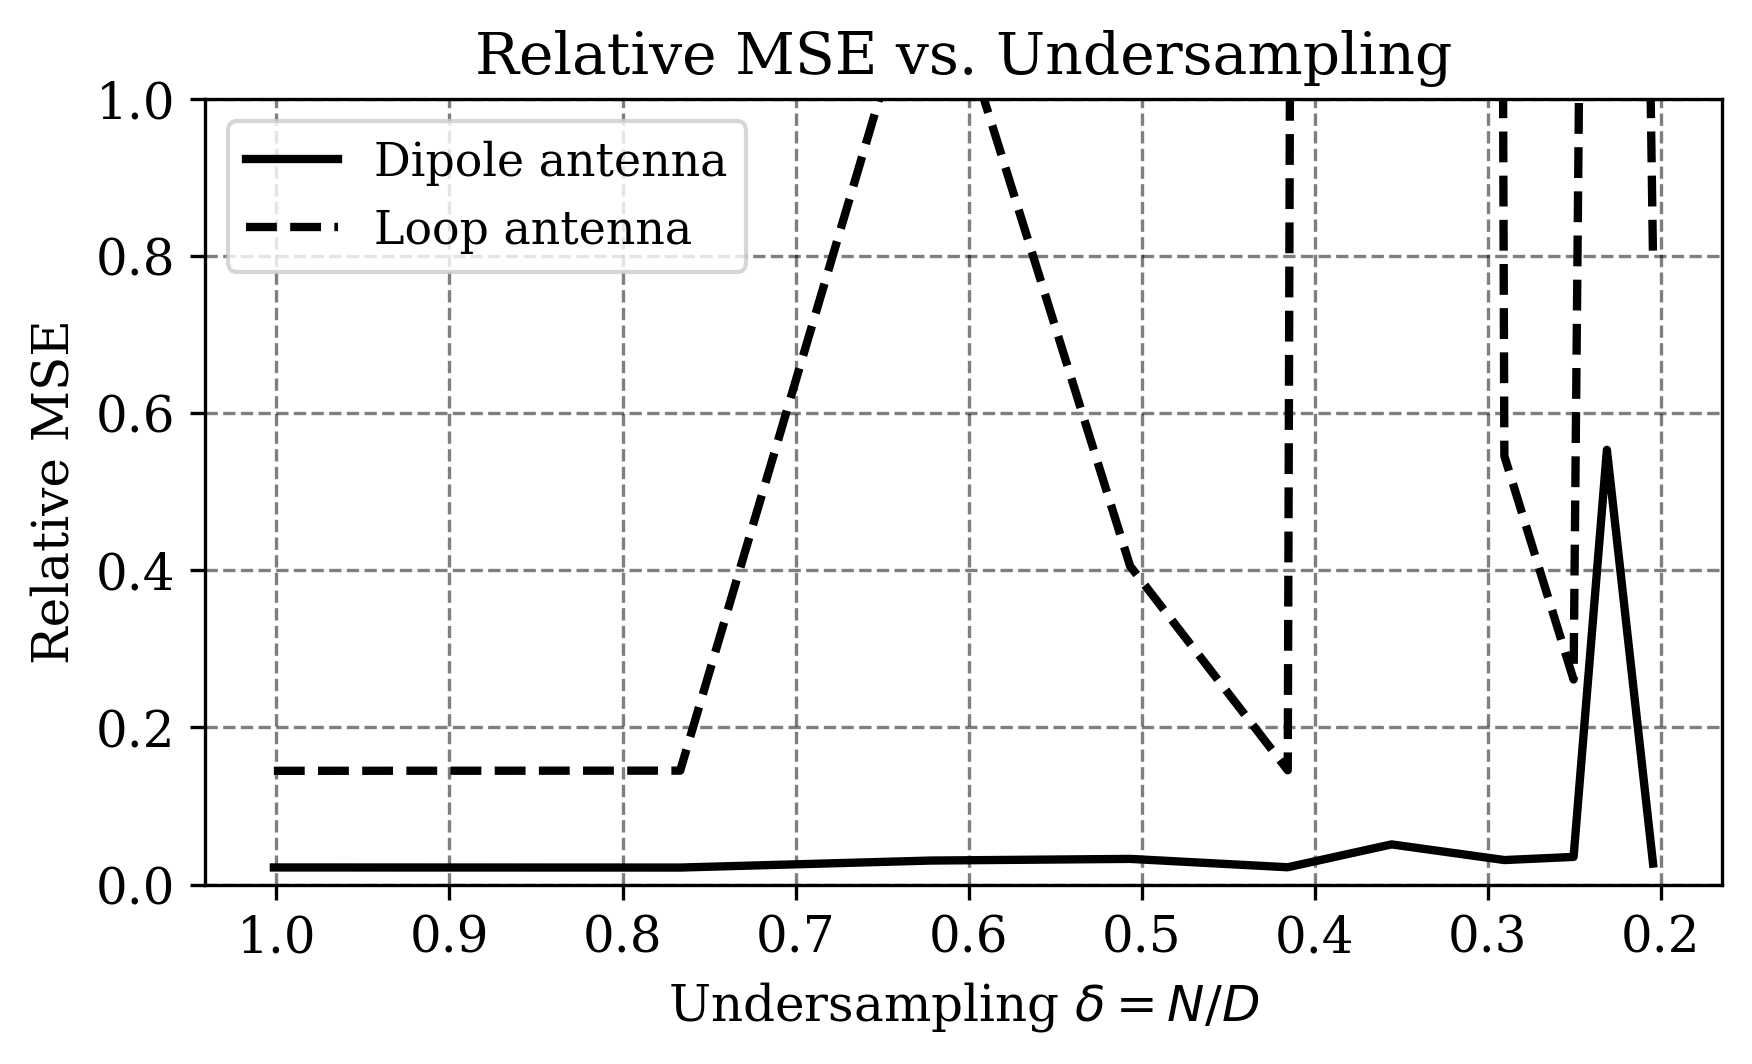
\includegraphics[width=0.75\linewidth]{Figures/delta_vs_mse_ff.png}
    \caption{Relative reconstruction error (normalized MSE) as a function of the measurement-to-dimension ratio $\delta = N/D$ for dipole and loop antennas in the far-field configuration.}
    \label{fig:mse_ff}
\end{figure}

In contrast, the dipole antenna exhibits robust reconstruction performance even under substantial undersampling, indicating that its radiation pattern is well-represented within the sparse spherical harmonics domain. However, the consistently higher reconstruction error for the loop antenna underscores the strong dependence of SBL performance on the specific radiation characteristics and topology of the source.

To further investigate the observed discrepancies and to validate the SBL results, a comparison was made between the coefficients obtained via the Fast Marginal Likelihood Algorithm and those computed through direct mode expansion using numerical integration, as theoretically described in Equation \ref{eq:expansion}. For the dipole antenna, there was a notable agreement between the dominant coefficients identified by both methods, as illustrated in Figure \ref{fig:dipole_weights}. This consistency supports the validity of the SBL-based estimation approach.

However, for the loop antenna, shown in Figure \ref{fig:loop_weights}, no such correspondence was observed. These results suggest either a fundamental difference in the sparsity structure of the loop antenna’s field representation or unresolved inaccuracies in the implementation of the spherical wave basis functions. A fully validated wave mode expansion method would have been essential for clarifying these observations; unfortunately, such a method could not be reliably implemented due to the challenges previously described.

\begin{figure}[H]
    \centering
    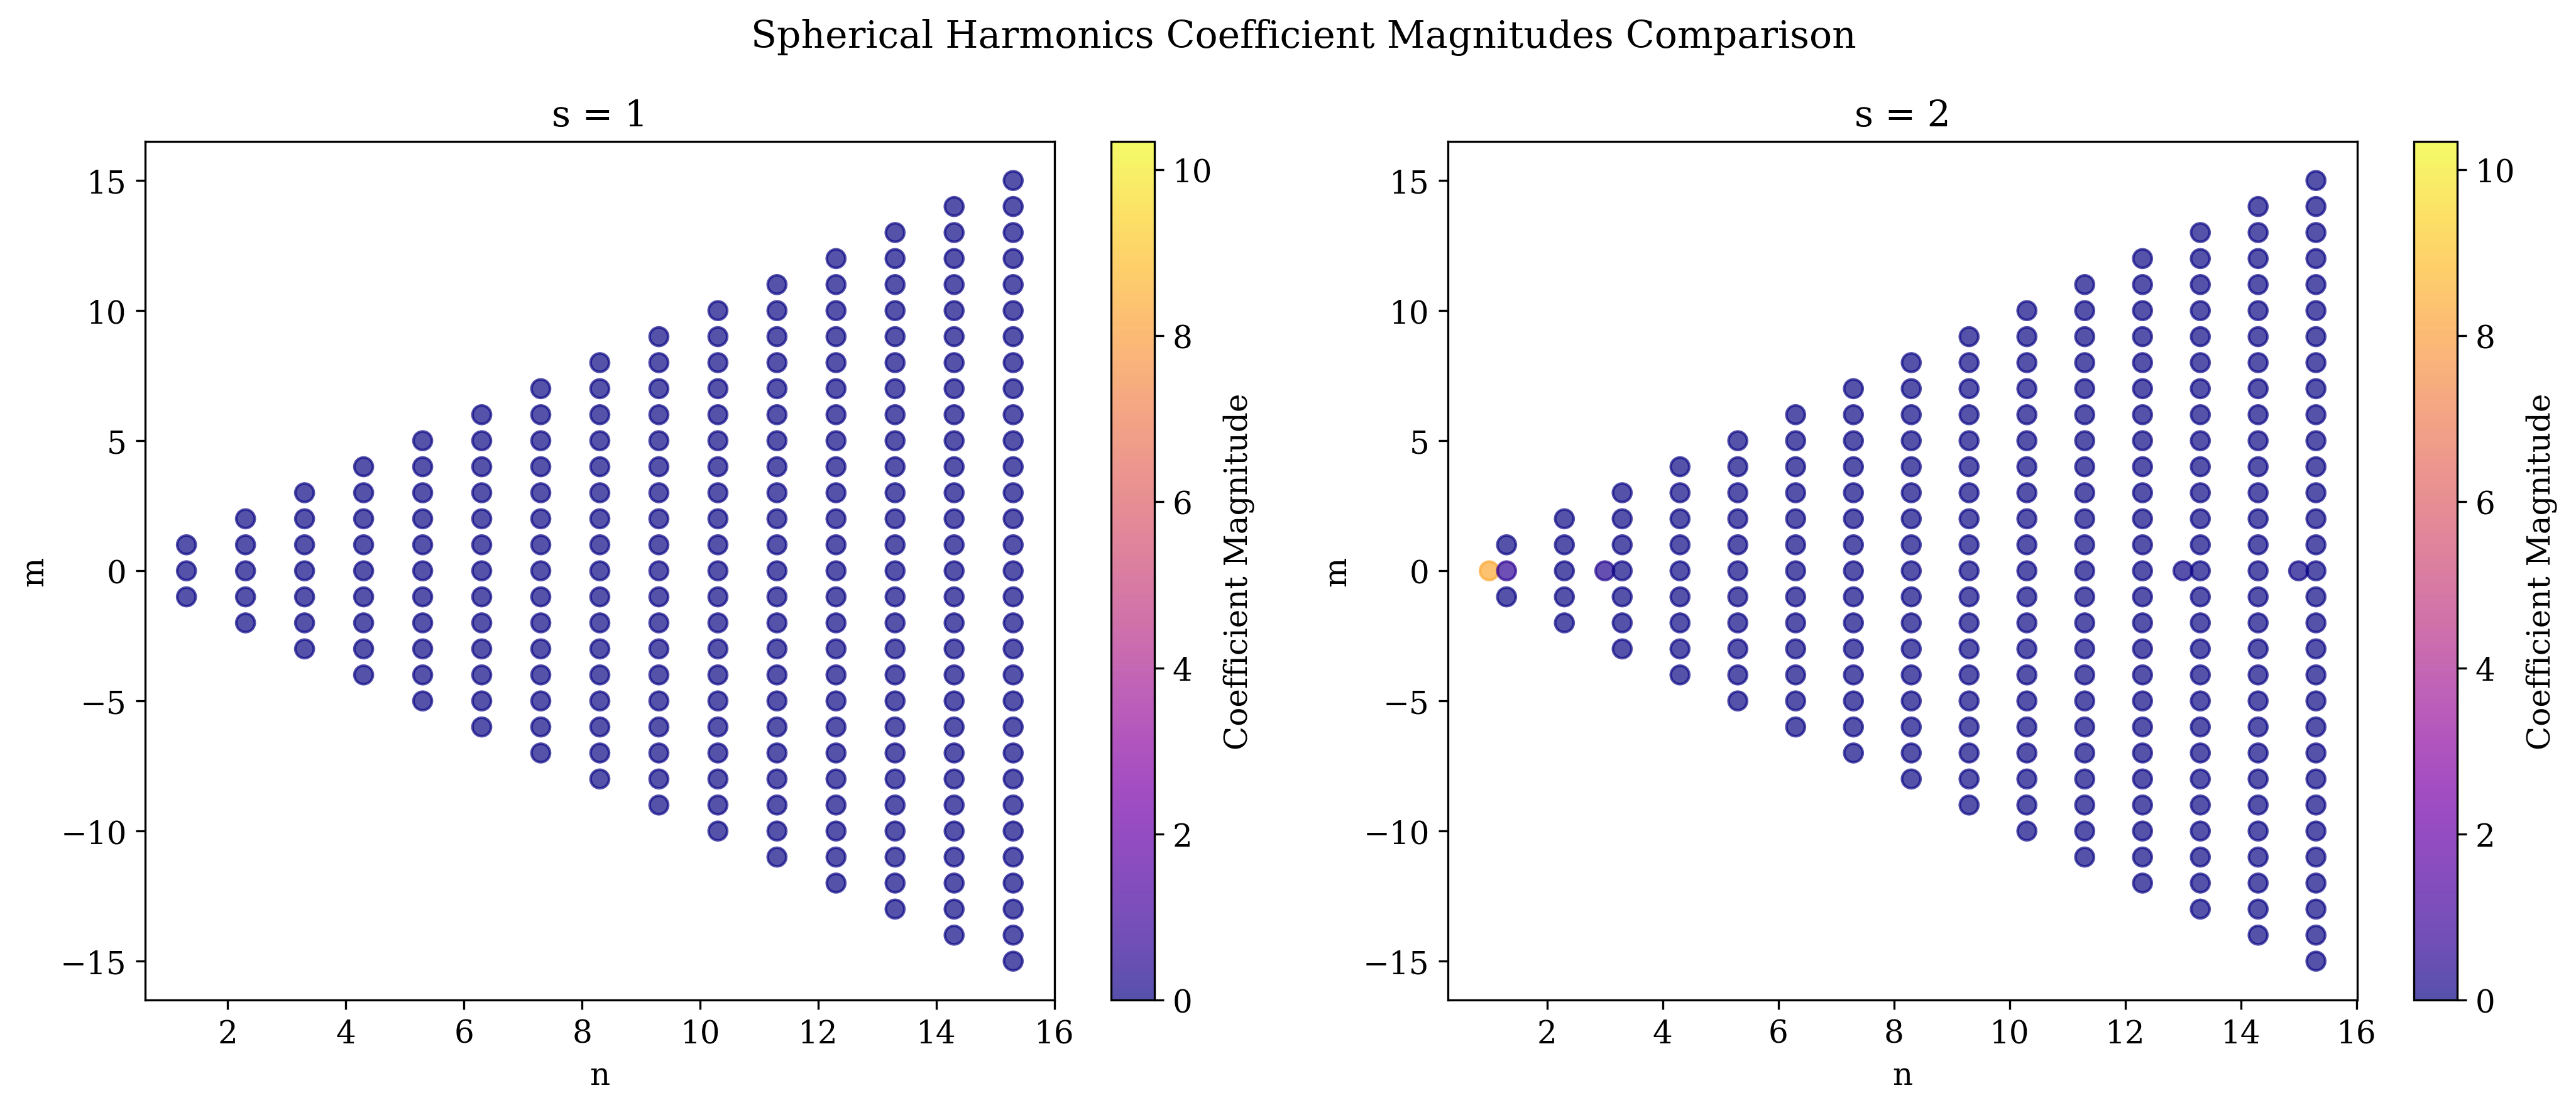
\includegraphics[width=1\linewidth]{Figures/dipole_ff_weights.png}
    \caption{Comparison of wave coefficients for the dipole antenna: non-zero weights estimated by the Fast Marginal Likelihood Algorithm (left) versus significant coefficients obtained via direct integration (right).}
    \label{fig:dipole_weights}
\end{figure}

\begin{figure}[H]
    \centering
    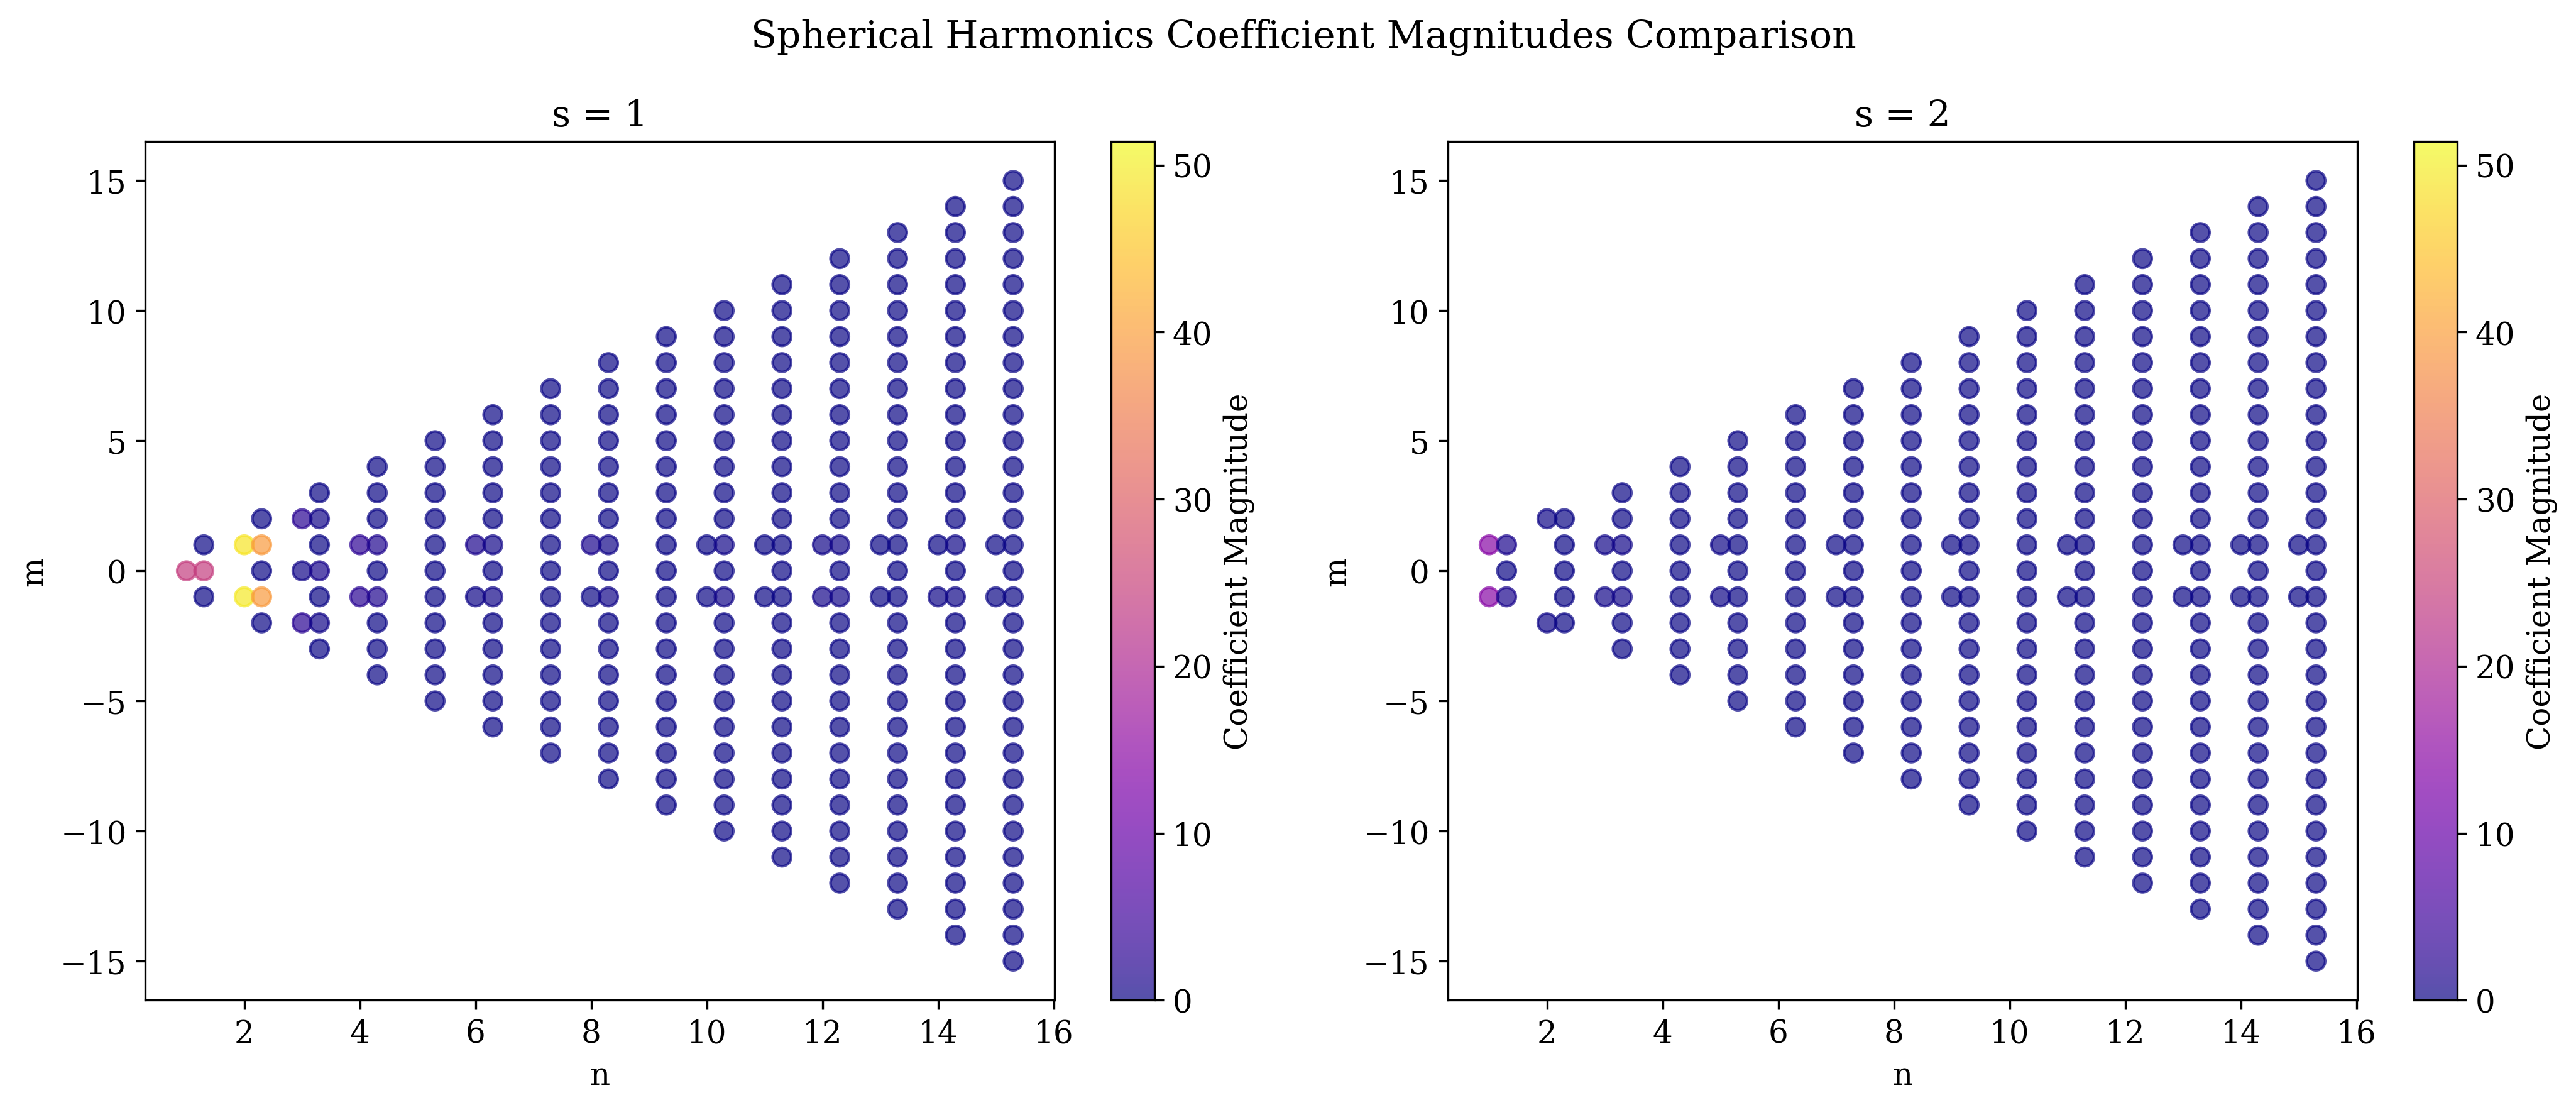
\includegraphics[width=1\linewidth]{Figures/loop_ff_weights.png}
    \caption{Comparison of wave coefficients for the loop antenna: non-zero weights estimated by the Fast Marginal Likelihood Algorithm (left) versus significant coefficients obtained via direct integration (right).}
    \label{fig:loop_weights}
\end{figure}


\bibliography{Compressive_Sensing_Report}

\end{document}
